% Options for packages loaded elsewhere
\PassOptionsToPackage{unicode}{hyperref}
\PassOptionsToPackage{hyphens}{url}
\PassOptionsToPackage{dvipsnames,svgnames,x11names}{xcolor}
%
\documentclass[
  a4paper,
]{scrreprt}

\usepackage{amsmath,amssymb}
\usepackage{iftex}
\ifPDFTeX
  \usepackage[T1]{fontenc}
  \usepackage[utf8]{inputenc}
  \usepackage{textcomp} % provide euro and other symbols
\else % if luatex or xetex
  \usepackage{unicode-math}
  \defaultfontfeatures{Scale=MatchLowercase}
  \defaultfontfeatures[\rmfamily]{Ligatures=TeX,Scale=1}
\fi
\usepackage{lmodern}
\ifPDFTeX\else  
    % xetex/luatex font selection
\fi
% Use upquote if available, for straight quotes in verbatim environments
\IfFileExists{upquote.sty}{\usepackage{upquote}}{}
\IfFileExists{microtype.sty}{% use microtype if available
  \usepackage[]{microtype}
  \UseMicrotypeSet[protrusion]{basicmath} % disable protrusion for tt fonts
}{}
\makeatletter
\@ifundefined{KOMAClassName}{% if non-KOMA class
  \IfFileExists{parskip.sty}{%
    \usepackage{parskip}
  }{% else
    \setlength{\parindent}{0pt}
    \setlength{\parskip}{6pt plus 2pt minus 1pt}}
}{% if KOMA class
  \KOMAoptions{parskip=half}}
\makeatother
\usepackage{xcolor}
\usepackage[top=2.5cm, bottom=2.5cm, left=3cm, right=3cm]{geometry}
\setlength{\emergencystretch}{3em} % prevent overfull lines
\setcounter{secnumdepth}{5}
% Make \paragraph and \subparagraph free-standing
\makeatletter
\ifx\paragraph\undefined\else
  \let\oldparagraph\paragraph
  \renewcommand{\paragraph}{
    \@ifstar
      \xxxParagraphStar
      \xxxParagraphNoStar
  }
  \newcommand{\xxxParagraphStar}[1]{\oldparagraph*{#1}\mbox{}}
  \newcommand{\xxxParagraphNoStar}[1]{\oldparagraph{#1}\mbox{}}
\fi
\ifx\subparagraph\undefined\else
  \let\oldsubparagraph\subparagraph
  \renewcommand{\subparagraph}{
    \@ifstar
      \xxxSubParagraphStar
      \xxxSubParagraphNoStar
  }
  \newcommand{\xxxSubParagraphStar}[1]{\oldsubparagraph*{#1}\mbox{}}
  \newcommand{\xxxSubParagraphNoStar}[1]{\oldsubparagraph{#1}\mbox{}}
\fi
\makeatother


\providecommand{\tightlist}{%
  \setlength{\itemsep}{0pt}\setlength{\parskip}{0pt}}\usepackage{longtable,booktabs,array}
\usepackage{calc} % for calculating minipage widths
% Correct order of tables after \paragraph or \subparagraph
\usepackage{etoolbox}
\makeatletter
\patchcmd\longtable{\par}{\if@noskipsec\mbox{}\fi\par}{}{}
\makeatother
% Allow footnotes in longtable head/foot
\IfFileExists{footnotehyper.sty}{\usepackage{footnotehyper}}{\usepackage{footnote}}
\makesavenoteenv{longtable}
\usepackage{graphicx}
\makeatletter
\newsavebox\pandoc@box
\newcommand*\pandocbounded[1]{% scales image to fit in text height/width
  \sbox\pandoc@box{#1}%
  \Gscale@div\@tempa{\textheight}{\dimexpr\ht\pandoc@box+\dp\pandoc@box\relax}%
  \Gscale@div\@tempb{\linewidth}{\wd\pandoc@box}%
  \ifdim\@tempb\p@<\@tempa\p@\let\@tempa\@tempb\fi% select the smaller of both
  \ifdim\@tempa\p@<\p@\scalebox{\@tempa}{\usebox\pandoc@box}%
  \else\usebox{\pandoc@box}%
  \fi%
}
% Set default figure placement to htbp
\def\fps@figure{htbp}
\makeatother
% definitions for citeproc citations
\NewDocumentCommand\citeproctext{}{}
\NewDocumentCommand\citeproc{mm}{%
  \begingroup\def\citeproctext{#2}\cite{#1}\endgroup}
\makeatletter
 % allow citations to break across lines
 \let\@cite@ofmt\@firstofone
 % avoid brackets around text for \cite:
 \def\@biblabel#1{}
 \def\@cite#1#2{{#1\if@tempswa , #2\fi}}
\makeatother
\newlength{\cslhangindent}
\setlength{\cslhangindent}{1.5em}
\newlength{\csllabelwidth}
\setlength{\csllabelwidth}{3em}
\newenvironment{CSLReferences}[2] % #1 hanging-indent, #2 entry-spacing
 {\begin{list}{}{%
  \setlength{\itemindent}{0pt}
  \setlength{\leftmargin}{0pt}
  \setlength{\parsep}{0pt}
  % turn on hanging indent if param 1 is 1
  \ifodd #1
   \setlength{\leftmargin}{\cslhangindent}
   \setlength{\itemindent}{-1\cslhangindent}
  \fi
  % set entry spacing
  \setlength{\itemsep}{#2\baselineskip}}}
 {\end{list}}
\usepackage{calc}
\newcommand{\CSLBlock}[1]{\hfill\break\parbox[t]{\linewidth}{\strut\ignorespaces#1\strut}}
\newcommand{\CSLLeftMargin}[1]{\parbox[t]{\csllabelwidth}{\strut#1\strut}}
\newcommand{\CSLRightInline}[1]{\parbox[t]{\linewidth - \csllabelwidth}{\strut#1\strut}}
\newcommand{\CSLIndent}[1]{\hspace{\cslhangindent}#1}

\usepackage{booktabs}
\usepackage{caption}
\usepackage{longtable}
\usepackage{colortbl}
\usepackage{array}
\usepackage{anyfontsize}
\usepackage{multirow}
\usepackage[font=small, labelfont={bf,small}, format=plain]{caption}
\makeatletter
\@ifpackageloaded{float}{}{\usepackage{float}}
\floatstyle{plain}
\@ifundefined{c@chapter}{\newfloat{suppfig}{h}{losuppfig}}{\newfloat{suppfig}{h}{losuppfig}[chapter]}
\floatname{suppfig}{Figure S}
\newcommand*\quartosuppfigref[1]{Figure \hyperref[#1]{S\ref{#1}}}
\@ifpackageloaded{caption}{}{\usepackage{caption}}
\DeclareCaptionLabelFormat{quartosuppfigreflabelformat}{#1#2}
\captionsetup[suppfig]{labelformat=quartosuppfigreflabelformat}
\newcommand*\listofsuppfigs{\listof{suppfig}{List of Supplementary Figures}}
\makeatother
\makeatletter
\@ifpackageloaded{bookmark}{}{\usepackage{bookmark}}
\makeatother
\makeatletter
\@ifpackageloaded{caption}{}{\usepackage{caption}}
\AtBeginDocument{%
\ifdefined\contentsname
  \renewcommand*\contentsname{Table of contents}
\else
  \newcommand\contentsname{Table of contents}
\fi
\ifdefined\listfigurename
  \renewcommand*\listfigurename{List of Figures}
\else
  \newcommand\listfigurename{List of Figures}
\fi
\ifdefined\listtablename
  \renewcommand*\listtablename{List of Tables}
\else
  \newcommand\listtablename{List of Tables}
\fi
\ifdefined\figurename
  \renewcommand*\figurename{Figure}
\else
  \newcommand\figurename{Figure}
\fi
\ifdefined\tablename
  \renewcommand*\tablename{Table}
\else
  \newcommand\tablename{Table}
\fi
}
\@ifpackageloaded{float}{}{\usepackage{float}}
\floatstyle{ruled}
\@ifundefined{c@chapter}{\newfloat{codelisting}{h}{lop}}{\newfloat{codelisting}{h}{lop}[chapter]}
\floatname{codelisting}{Listing}
\newcommand*\listoflistings{\listof{codelisting}{List of Listings}}
\makeatother
\makeatletter
\makeatother
\makeatletter
\@ifpackageloaded{caption}{}{\usepackage{caption}}
\@ifpackageloaded{subcaption}{}{\usepackage{subcaption}}
\makeatother

\usepackage{bookmark}

\IfFileExists{xurl.sty}{\usepackage{xurl}}{} % add URL line breaks if available
\urlstyle{same} % disable monospaced font for URLs
\hypersetup{
  pdftitle={Expression Profiling of Differentially Expressed Genes Under Stress Conditions and FLC1 Modulation in Cryptococcus neoformans},
  pdfauthor={Diego Cesar Villa Almeyda},
  colorlinks=true,
  linkcolor={blue},
  filecolor={Maroon},
  citecolor={Blue},
  urlcolor={Blue},
  pdfcreator={LaTeX via pandoc}}


\title{Expression Profiling of Differentially Expressed Genes Under
Stress Conditions and FLC1 Modulation in \emph{Cryptococcus neoformans}}
\author{Diego Cesar Villa Almeyda}
\date{July, 2025}

\begin{document}
\cleardoublepage
\thispagestyle{empty}
\vspace*{2cm}  % Adds top space, adjust as needed

\begin{center}
  {\huge\bfseries Expression Profiling of Differentially Expressed Genes
Under Stress Conditions and FLC1 Modulation in \emph{Cryptococcus
neoformans} \par}
    
  \vspace{6em}

    {\Large\bfseries Diego Cesar Villa Almeyda \par}
  
  \vspace{2em}
  {\bfseries\large Master of Science \par}
  
  \vspace{1.5em}
  {\bfseries\large July, 2025 \par}
  
  \vspace{4em}

      {\bfseries\large School of Mathematics \par}
    
  {\bfseries\large The University of Edinburgh \par}
      
  \vspace{6em}
  {\small Dissertation Presented for the Degree of MSc in Statistics with Data Science \par}
\end{center}

\renewcommand*\contentsname{Table of contents}
{
\hypersetup{linkcolor=}
\setcounter{tocdepth}{2}
\tableofcontents
}

\bookmarksetup{startatroot}

\chapter*{Own work declaration}\label{own-work-declaration}
\addcontentsline{toc}{chapter}{Own work declaration}

\markboth{Own work declaration}{Own work declaration}

\textbf{Name}: Diego Cesar Villa Almeyda

\textbf{Matriculation Number}: S2750743

\textbf{Title of work}: Differential Gene Expression in
\emph{Cryptococcus neoformans} Cell Wall Stress Response

I confirm that all this work is my own except where indicated, and that
I have:

\begin{itemize}
\tightlist
\item
  Clearly referenced/listed all sources as appropriate.\\
\item
  Referenced and put in inverted commas all quoted text (from books,
  web, etc)\\
\item
  Given the sources of all pictures, data etc. that are not my own.\\
\item
  Not made any use of the report(s) or essay(s) of any other student(s)
  either past\\
  or present.
\item
  Not sought or used the help of any external professional academic
  agencies for the work.
\item
  Acknowledged in appropriate places any help that I have received from
  others (e.g.~fellow students, technicians, statisticians, external
  sources).
\item
  Complied with any other plagiarism criteria specified in the Course
  handbook.
\end{itemize}

I understand that any false claim for this work will be penalised in
accordance with the University regulations
(https://teaching.maths.ed.ac.uk/main/msc-students/msc-programmes/statistics/data-science/assessment/academic-misconduct){[}https://teaching.maths.ed.ac.uk/main/msc-students/msc-programmes/statistics/data-science/assessment/academic-misconduct{]}.

Signature:

\includegraphics[width=0.2\linewidth,height=\textheight,keepaspectratio]{figures/signature.jpg}

Date: 1st July 2025

\bookmarksetup{startatroot}

\chapter*{Executive summary}\label{executive-summary}
\addcontentsline{toc}{chapter}{Executive summary}

\markboth{Executive summary}{Executive summary}

This report analyses RNA-seq data from an experiment designed to
understand how \emph{Cryptococcus neoformans} responds to cell wall
stress under varying genetic and environmental conditions, with a focus
on the FLC1 gene, a candidate antifungal drug target. Cells from
wild-type and FLC1Δ strains were grown under combinations of temperature
(30°C or 37°C) and growth media (YPD, with or without CFW and/or EGTA),
simulating stress conditions.

The analysis confirmed strong biological replicate consistency of the
experimental data and revealed that strain background shaped the
response to stress: FLC1Δ cells displayed more pronounced expression
changes, particularly in response to CFW and at higher temperatures. Key
driver genes of this variation included FLC1 gene itself (CNAG\_04283),
as well as CNAG\_01653, CNAG\_04891, and CNAG\_00588.

Differential expression analysis identified over 3,400 genes (52.4\%)
with significant changes related to the interaction of the experimental
factors, especially when contrasting the FLC1Δ strain under compound
stress (CFW + EGTA at 37°C) with the wild-type strain under basal medium
at 37°C, where most were downregulated. One gene, CNAG\_06576, showed
consistent high significance and condition-specific regulation.
Clustering the top 500 most informative DE genes revealed four major
expression patterns, primarily driven by strain and stress condition,
with one cluster reflecting stress-induced repression in the mutant
FLC1Δ strain.

The findings suggest FLC1 plays a key role in mediating the
transcriptional stress response. A ranked list of the top 100 DE genes
is provided for future functional characterisation. While robust, the
results are based on a single DE method (\texttt{DESeq2}), and could be
further validated using complementary statistical methods.

\bookmarksetup{startatroot}

\chapter{Introduction}\label{introduction}

\emph{Cryptococcus neoformans} is a globally distributed fungal pathogen
responsible for hundreds of thousands of deaths annually, mainly
affecting immunocompromised individuals (1). Treatment options are
limited and increasingly compromised by drug resistance, with all major
antifungal classes (polyenes, azoles, and pyrimidine analogues) facing
challenges related to toxicity and reduced efficacy. This high disease
burden, coupled with rising antifungal resistance, highlights an urgent
need for novel therapeutic strategies.

Recent studies have identified the FLC1 protein as a critical factor in
\emph{C. neoformans} stress response and virulence (2). Because FLC1
homologues are present in other fungal pathogens but poorly conserved in
humans, it presents a promising drug target that could enable
broad-spectrum antifungal therapies with reduced host toxicity.
Motivated by this, the present report analyses transcriptomic data from
an experiment by Rachel Murray (Wallace Lab, University of Edinburgh)
exploring fungal responses to cell wall stressors---calcofluor white
(CFW), EGTA (a calcium chelator), and deletion of FLC1, which is
implicated in calcium import. Preliminary observations showed that FLC1
deletion causes abnormal cell wall morphology and lethality at 37°C,
effects that EGTA can suppress. This analysis aims to uncover the gene
expression changes underlying these phenotypes and provide a statistical
foundation for further biological insights.

RNA sequencing (RNA-Seq) is a high-throughput technology that enables
accurate, genome-wide profiling of gene expression and transcript
isoforms at single-base resolution (3). In the described experiment,
RNA-Seq measured transcript abundance across thousands of genes after a
3-hour incubation under varying environmental (growth media and
temperature) and genetic (presence or deletion of FLC1) conditions.

Our analysis of this RNA-Seq data had three main goals: (i) assess
replicate quality and explore broad expression patterns across samples;
(ii) identify genes differentially expressed in response to
environmental or genetic changes; and (iii) characterise distinct
expression patterns within these differentially expressed genes. These
efforts provide robust statistical evidence to guide further biological
interpretation and prioritise candidate genes for functional studies of
cell wall stress mechanisms in \emph{C. neoformans}.

\bookmarksetup{startatroot}

\chapter{Methods}\label{sec-methods}

\section{Experimental design and data}\label{sec-data}

\begin{table}

\caption{\label{tbl-01}Overview of the experimental design showing the
combinations of temperature and growth media (environmental conditions)
used to grow cells of the WT and FLC1Δ (FL) strains. Each cell lists the
replicate sample labels (S1--S30) corresponding to each unique
experimental condition.}

\centering{

\fontsize{7.5pt}{9.0pt}\selectfont
\begin{tabular*}{0.8\linewidth}{@{\extracolsep{\fill}}cccccc}
\toprule
 & \multicolumn{5}{c}{\textbf{Enviromental conditions}} \\ 
\cmidrule(lr){2-6}
 & \textbf{30°C} & \multicolumn{4}{c}{\textbf{37°C}} \\ 
\cmidrule(lr){2-2} \cmidrule(lr){3-6}
\textbf{Strain} & \textbf{Y} & \textbf{Y} & \textbf{YC} & \textbf{YE} & \textbf{YCE} \\ 
\midrule\addlinespace[2.5pt]
WT & S1, S2, S3 & S4, S5, S6 & S7, S8, S9 & S10, S11, S12 & S13, S14, S15 \\ 
FL & S16, S17, S18 & S19, S20, S21 & S22, S23, S24 & S25, S26, S27 & S28, S29, S30 \\ 
\bottomrule
\end{tabular*}

}

\end{table}%

The study involved culturing cells from both the wild-type (WT, FLC1
gene present) and FLC1Δ (FL, FLC1 gene absent) strains under various
environmental conditions. Cells were grown in four different growth
medium: YPD (Y), YPD with CFW (YC), YPD with EGTA (YE), and YPD with
both CFW and EGTA (YCE), all at 37°C to induce stress. Additionally,
both strains were grown under baseline conditions in standard YPD at
30°C. In total, 10 distinct experimental conditions were tested (5
environmental conditions × 2 strains), each with 3 biological
replicates, resulting in 30 samples.

Table~\ref{tbl-01} presents the experimental design along with the
sample labels for each condition. The 10 experimental conditions are
labeled by combining the levels of the three experimental factors:
strain, temperature, and growth media, in that order. For example, the
condition involving the wild-type strain grown in YCE medium at 37°C is
labeled WT-37-YCE, while the corresponding condition for the FLC1Δ
strain is labeled FL-37-YCE.

The primary output of the experiment was a raw count matrix containing
RNA abundance measurements for 6795 genes across 30 samples, resulting
in a 6795 × 30 matrix. Each entry in the matrix represents the number of
sequencing reads mapped to a specific gene in a given sample.

\section{Pre-filtering}\label{sec-filter}

Genes with consistently low or zero counts across samples are unlikely
to be biologically active and are typically excluded before DE analysis.
This pre-filtering step is justified because genes must surpass a
minimal expression threshold to produce functional proteins or exert
biological effects (4), and low counts often reflect sampling noise
rather than true signal (5).

Filtering also improves statistical power. Since DE analysis tests each
gene for expression differences between conditions, it involves multiple
hypothesis testing, typically corrected via FDR adjustment. These
corrections reduce power, especially when many genes are tested but few
are truly DE (6). Removing low-expression genes reduces the number of
tests, making FDR correction less stringent and increasing the
likelihood of detecting true positives (5,6).

Although the software used for differential expression (DE) analysis
includes an internal filtering routine (see Section~\ref{sec-de}),
additional pre-filtering was applied using an empirical method
implemented in the R package \texttt{edgeR} (7), as described in (4).
This method retains genes whose counts-per-million (CPM) exceed a
specified threshold \(k\) in at least \(n\) samples. The CPM for each
gene in a sample is calculated by dividing the raw read count by the
total number of reads (i.e., the library size) in that sample and
scaling by one million.

To determine the CPM threshold \(k\), the user specifies a minimum raw
count that a gene must meet in \(n\) samples, and the software computes
the corresponding CPM based on the smallest library size. For this
study, we required a minimum count of 10 in at least 3 samples,
corresponding to the number of replicates per condition. The original,
unfiltered count matrix was retained to replicate the DE analysis and
compare results.

\section{Normalisation and transformation}\label{sec-norm}

In RNA-seq experiments, raw read counts are influenced by both gene
expression and technical factors, such as library size, gene length, and
GC content, making them not directly comparable across samples or genes
(8,9). Between-sample variation, mainly due to differences in library
size, is commonly corrected using normalisation methods.

While total count normalisation (e.g., CPM) adjusts for library size, it
can be biased by a few highly expressed genes, potentially distorting
the expression estimates of others and introducing artefactual
differences (8). More robust approaches like TMM have been proposed
(10). In this study, we used the \texttt{DESeq2} median-of-ratios method
to estimate sample-specific size factors (11,12), and CPM was also
applied for comparison. Within-sample normalisation (e.g., for gene
length or GC content) was not performed, following the project advisor's
recommendation.

RNA-seq data visualisation and multivariate analyses like clustering or
PCA are sensitive to heteroskedasticity, where genes with higher
expression tend to show greater variance. This can allow highly
expressed genes to dominate the analysis and obscure biological signals
(12). Variance-stabilising transformations (VSTs) are often used to
place genes on a comparable scale (13).

Log transformation is a common approach but tends to exaggerate
variability in low-count genes, where noise can dominate (12). In this
study, we applied the regularised log (rlog) and VST methods implemented
in \texttt{DESeq2} (11,12), both applied after \texttt{DESeq2}
normalisation. For comparison, we also used a base-2 log transformation
on CPM-normalised counts, with a prior count of 2 to avoid undefined
values.

Transformations were assessed using mean--SD plots for gene-wise
variance and boxplots of sample expression profiles to evaluate the
extent of variance stabilisation.

\section{Exploratory analysis}\label{seq-eda}

An important early step in RNA-seq analysis is assessing the quality and
consistency of biological replicates. Ideally, replicates under the same
condition should show similar expression profiles after normalisation
and transformation. To evaluate this, we used principal component
analysis (PCA) to project samples into a lower-dimensional space and
examine whether replicates cluster together. PCA decomposes the
expression matrix into uncorrelated components ordered by the variance
they explain, offering a visual summary of sample similarity. We applied
Horn's parallel analysis to determine how many components to retain,
comparing observed eigenvalues to those from randomly generated data and
keeping components that exceeded the simulated average (14). This
analysis was performed on three transformed datasets: log-transformed
CPM, rlog-transformed counts, and VST-transformed counts, as described
in Section~\ref{sec-norm}.

To visualise sample structure and identify genes contributing to
variation, we generated PCA biplots showing the samples along with the
five genes most strongly correlated with each principal component, based
on their loadings. Loading plots displaying the top 10 of genes by
absolute loading value were also produced. To explore the relationship
between experimental conditions and the principal components, we
conducted ANOVA tests on the component scores, using each experimental
factor as a grouping variable. All PCA analyses were performed using the
top 10\% most variable genes, which are more likely to reflect
meaningful biological signals, while low-variance genes were excluded as
typically uninformative.

\section{Differential expression analysis}\label{sec-de}

The DE analysis approach used in this study follows the methodology
implemented in the \texttt{DESeq2} package. The core idea is to model
the raw counts for each gene using a negative binomial (NB)
distribution, where the logarithm of the normalised mean is modeled as a
linear combination of coefficients corresponding to contrasts of
experimental conditions. Hypothesis testing is then performed on these
coefficients to assess whether the corresponding contrasts result in
statistically significant differential expression for a given gene. In
the remainder of this section, we briefly outline the key features of
this modeling framework, as described in (12).

Let \(c_{ij}\) denote the observed raw count for gene \(i\) in sample
\(j\). We assume that \(c_{ij}\) has a NB distribution with mean
\(\mu_{ij}\) and gene-specific dispersion parameter \(\alpha_i\); that
is, \(c_{ij} \sim \mathcal{NB}(\mu_{ij}, \alpha_i)\). The mean
\(\mu_{ij}\) is modelled as the product of a sample-specific size factor
\(s_j\) and a normalised expression level \(q_{ij}\), such that
\(\mu_{ij} = s_j q_{ij}\). The size factor \(s_j\) is estimated using
the median-of-ratios method, as mentioned in Section~\ref{sec-norm}.
Finally, the dispersion parameter is used to model the variance of the
counts via \(\text{var}(c_{ij}) = \mu_{ij}+\alpha_i\mu_{ij}^2\).

The log-transformation of the normalised expression level, \(q_{ij}\),
is modelled in this study as

\begin{equation}\phantomsection\label{eq-glm}{
\begin{aligned}
\text{log}(q_{ij}) &= \beta_{i0} + \beta_{i1}x^{(\text{FL})}_{j} + \beta_{i2}x^{(\text{YC})}_{j} + \beta_{i3}x^{(\text{YE})}_{j} + \beta_{i4}x^{(\text{YCE})}_{j} + \beta_{i5}x^{(\text{30})}_{j} + \\
& \quad \quad \beta_{i6}x^{(\text{FL})}_{j}x^{(\text{YC})}_{j} + \beta_{i7}x^{(\text{FL})}_{j}x^{(\text{YE})}_{j} + \beta_{i8}x^{(\text{FL})}_{j}x^{(\text{YCE})}_{j} + \beta_{i9}x^{(\text{FL})}_{j}x^{(\text{30})}_{j},
\end{aligned}
}\end{equation}

where the intercept term \(\beta_{i0}\) denotes the baseline expression
level of gene \(i\) under the reference condition. The coefficients
\(\beta_{i1}\) to \(\beta_{i5}\) represent the main effects of the
experimental factors: \(x^{(\text{FL})}_{j}\) is an indicator variable
for the FLC1Δ strain, with the WT strain serving as the reference level;
\(x^{(\text{YC})}_{j}\), \(x^{(\text{YE})}_{j}\), and
\(x^{(\text{YCE})}_{j}\) are indicators for the different media
conditions, with Y as the reference level; and \(x^{(\text{30})}_{j}\)
indicates the 30°C temperature condition, with 37°C as reference.
Together, this implies that the reference experimental condition is
WT-37-Y. The interaction terms \(\beta_{i6}\) to \(\beta_{i9}\) model
how the effects of media and temperature differ under the presence or
absence of the FLC1 gene. No interaction between media and temperature
was included, as these factors are not fully crossed in the experimental
design.

Accurate estimation of gene-specific dispersion parameters
(\(\alpha_i\)) is essential for reliable differential expression
analysis. However, in experiments with small sample sizes---such as this
one---maximum likelihood estimates (MLE) of dispersion can be highly
variable and compromise significance testing (12). To address this,
\texttt{DESeq2} applies an empirical Bayes shrinkage approach that pulls
dispersion estimates toward a trend based on mean expression. This trend
is derived from gene-wise estimates and modelled using a parametric
regression, with final dispersion values obtained as maximum a
posteriori (MAP) estimates under a log-normal prior. In cases where the
gene-wise estimate notably exceeds the trend, \texttt{DESeq2} retains
the original estimate to avoid underestimating true variance and
inflating false positives.

The log-fold change (LFC), typically expressed on a \(\text{log}_2\)
scale, represents the change in gene expression between two conditions
and corresponds to the model coefficients in Equation~\ref{eq-glm},
estimated via MLE using the shrunken dispersion values. However,
MLE-derived LFCs can be highly variable, especially for low-count genes.
To improve their stability and interpretability, \texttt{DESeq2} applies
an empirical Bayes shrinkage procedure introduced by (15) and
implemented in the \texttt{apeglm} package. This approach uses a
heavy-tailed Cauchy prior, with the prior scale adaptively estimated
from the data, and produces MAP estimates that combine the negative
binomial likelihood with the prior. Uncertainty is quantified using a
Laplace approximation to the posterior. Although this shrinkage does not
affect which genes are identified as significantly differentially
expressed, it yields more reliable effect size estimates for downstream
analyses such as visualisation, gene filtering, and functional
enrichment (16).

In \texttt{DESeq2}, differential expression is assessed using a Wald
test on the maximum likelihood estimates of log-fold changes (LFCs),
testing the null hypothesis \(H_0: \beta_{ik} = 0\) against the
alternative \(\beta_{ik} \neq 0\). Although a zero LFC may be
biologically unlikely due to complex gene regulatory networks, it
provides a practical baseline for statistical testing, especially in
small-scale studies like ours with only three replicates per condition
(12). P-values are adjusted for multiple testing using the
Benjamini--Hochberg procedure to control the false discovery rate (FDR)
(17). Due to limited statistical power, we use an adjusted p-value
threshold of 0.1 to determine significance.

As discussed in Section~\ref{sec-filter}, \texttt{DESeq2} performs
independent filtering by default, using the mean of normalised counts to
exclude genes with low expression. The filtering threshold is
automatically chosen to maximise discoveries at the target false
discovery rate (FDR), set here at 0.1. This filter is independent of the
test statistic under the null hypothesis, enhancing statistical power
(6). Additionally, \texttt{DESeq2} incorporates automatic outlier
detection based on Cook's distance, flagging observations exceeding the
99th percentile of the \(F(q, q-n)\) distribution, where \(q\) is the
number of model parameters and \(n\) the number of samples. Outlier
handling depends on sample size: it is skipped for conditions with two
or fewer replicates; genes with outliers are excluded when there are six
or fewer replicates; and for seven or more replicates, outliers are
replaced with imputed values via trimmed means before refitting the
model.

The rlog transformation, introduced in Section~\ref{sec-norm}, converts
raw counts \(c_{ij}\) for gene \(i\) in sample \(j\) to
\(\log_2(q_{ij}) = \beta_{i0} + \beta_{ik}\), fitting a model similar to
Equation~\ref{eq-glm} and applying empirical Bayes shrinkage to the
log-fold changes relative to baseline expression \(\beta_{i0}\). By
default, \texttt{DESeq2} uses blind dispersion estimation for rlog,
ignoring experimental design and treating all samples as replicates of a
single condition. This makes rlog-transformed data suitable for
unsupervised analyses like quality control, minimizing experimental
group effects. The VST transformation is also blinded by default.

Our downstream analysis focused on the four interaction terms
\(\beta_{i6}\) to \(\beta_{i9}\) in Equation~\ref{eq-glm} to identify
genes whose stress response is modulated by the presence or absence of
the FLC1 gene, while also considering main effects. To assess model fit,
we examined the dispersion plot, expecting gene-wise dispersions to
scatter around the fitted mean-dependent trend, with dispersion
decreasing as mean expression increases (16). After multiple testing,
the p-value distribution was inspected; a well-calibrated test should
show a spike near zero and a flat distribution elsewhere (18). We
produced MA plots for both unshrunken and shrunken LFCs, highlighting
significant and non-significant genes to visualise fold change magnitude
and distribution across expression levels (16). Volcano plots displayed
the top 10 most significant genes by adjusted p-value.

We compared the significant gene sets for the interaction terms by
assessing both the number of genes per interaction and their overlaps.
To identify shared expression patterns, we selected the top 500 most
variable genes across samples for all interactions and performed
hierarchical clustering on the correlation matrix of z-scores derived
from normalised counts. For this, rlog and VST transformations were
applied without blinding, using the design matrix to estimate
dispersions. The optimal cluster number was determined via the Gap
statistic (19). Cluster expression profiles were visualised through
heatmaps and line plots to illustrate expression trends across
experimental conditions.

\section{Software}\label{software}

All analyses were performed using R version 4.4.1. Differential
expression analysis was conducted with the \texttt{DESeq2} package,
version 1.46.0. The complete code for reproducing the analysis and
generating this report is available at
\url{https://github.com/dievillano/gene-expression}.

\bookmarksetup{startatroot}

\chapter{Results}\label{sec-results}

Gene-wise total read counts ranged from 0 to 2.97 million, with gene
CNAG\_06125 showing the highest total count across all samples. A total
of 25 out of 6795 genes had zero total counts. Library sizes (i.e.,
total read counts per sample) ranged from 4.26 to 9.02 million, with
sample S12 from condition FL-Y-37 having the largest library. At the
condition level, WT-Y-30 showed the highest total library size (25.93
million). A barplot of library sizes across samples is shown in
\quartosuppfigref{suppfig-libsize}, highlighting variability across
libraries and the need for normalisation prior to comparing expression
levels.

\section{Pre-processing}\label{pre-processing}

After pre-filtering, we retained 6613 genes (97.32\%), removing 182
genes and moderately reducing the multiple testing burden for DE
analysis. We applied CPM normalisation followed by \(\text{log}_2\)-CPM,
rlog, and VST transformations on the filtered count matrix as described
in Section~\ref{sec-norm}. \quartosuppfigref{suppfig-boxplots} presents
boxplots of expression values by sample and condition for each
transformation. CPM alone did not stabilise variance, showing skewed
distributions with many outliers. In contrast, \(\text{log}_2\)-CPM,
rlog, and VST reduced skewness and improved centring, though some
outliers remain. Among these, rlog and VST yielded more uniform
distributions across samples compared to the simple log transform, which
has known limitations (see Section~\ref{sec-norm}). The impact on
variance stabilisation is further illustrated in
\quartosuppfigref{suppfig-meansd}, which plots gene-wise standard
deviations against ranked mean expression for each transformation. CPM
displays a pronounced variability peak at high expression levels,
whereas transformed data show flatter trends, indicating effective
variance stabilisation across the expression range.

\section{Quality assessment and exploratory
analysis}\label{quality-assessment-and-exploratory-analysis}

PCA was performed on the transformed data of the genes at the 10\% of
highest variance, yielding an optimal number of three components for all
methods except CPM, which retained only one. These components explained
92.86\%, 93.19\%, and 92.71\% of the total variance for \(\log_2\)-CPM,
rlog, and VST, respectively, while CPM explained only 75.19\%. The scree
plot for the rlog-transformed data, shown in
\quartosuppfigref{suppfig-scree}, illustrates the retained components
and their associated variance. The score plots for all retained
component pairs in \quartosuppfigref{suppfig-pca-rlog} show that
replicates from the same condition cluster tightly, indicating high
consistency and replicate quality. Since the rlog and VST
transformations yield similar explained variance (slightly higher for
rlog) we will present results based on the rlog-transformed data from
this point forward.

\begin{figure}

\centering{

\pandocbounded{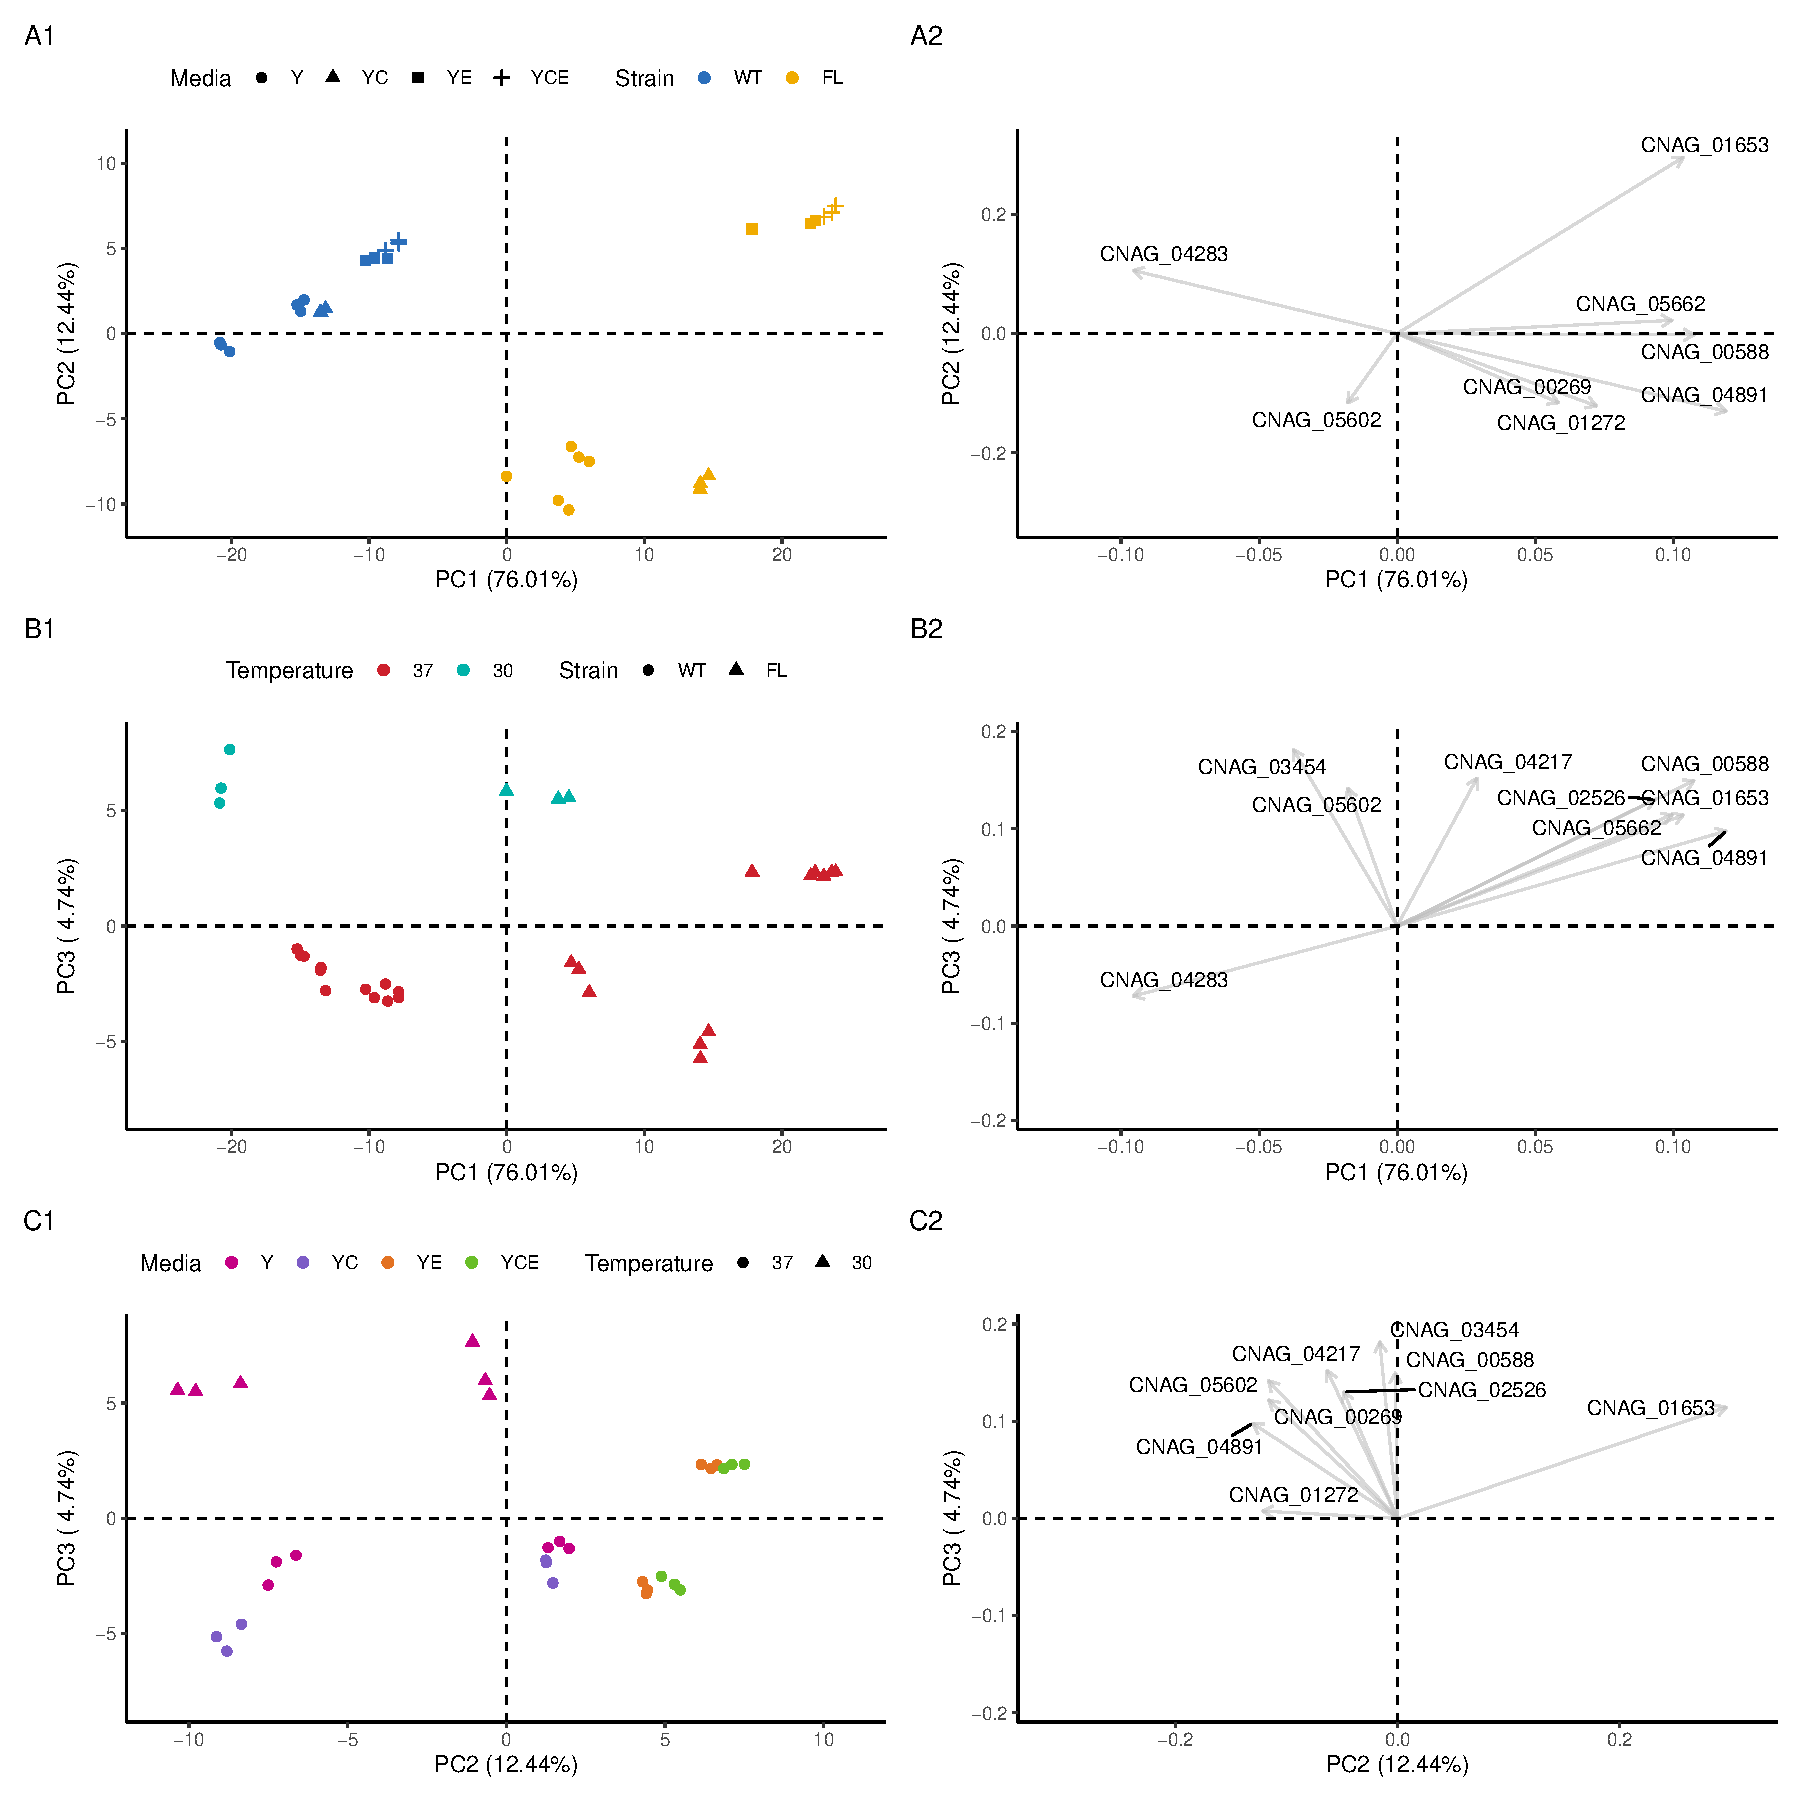
\includegraphics[keepaspectratio]{figures/pca_rlog_full_plot.pdf}}

}

\caption{\label{fig-pca-rlog-full}Sample projections onto pairs of
principal components: (A) PC1 vs PC2, (B) PC1 vs PC3, and (C) PC2 vs
PC3. Subplots labeled 1 display sample scores coloured and shaped by
relevant experimental conditions, while subplots labeled 2 show loadings
of the top 10 genes with the highest absolute loadings on each component
pair.}

\end{figure}%

In Figure~\ref{fig-pca-rlog-full}, subplot A1, samples separate clearly
by strain along PC1 and by media condition along PC2. Notably, samples
from conditions Y and YC, as well as YE and YCE, cluster closely
together, suggesting that EGTA primarily drives the observed separation
rather than CFW. This distinction between samples with and without EGTA
is more pronounced in the FLC1Δ strain compared to the WT strain.
Additionally, a clear separation between samples grown in Y and YC media
is observed only for the FLC1Δ strain, indicating a potential
interaction between strain and growth media.

Subplot A2 shows that genes CNAG\_04283 and CNAG\_05602 mainly drive
separation toward the WT strain, with CNAG\_04283 having the strongest
effect as expected since it corresponds to the FLC1 gene itself. Genes
CNAG\_05662 and CNAG\_00588 align closely with FLC1Δ samples, while
CNAG\_00269, CNAG\_01272, and CNAG\_04891 appear to contribute to the
separation of FLC1Δ samples grown in Y and YC media. Notably,
CNAG\_01653 is strongly associated with FLC1Δ samples grown with EGTA,
suggesting a gene-specific response to this condition.

In subplot B1, samples separate by temperature along PC3, with further
strain-specific separation within each temperature group, suggesting a
potential interaction between these factors. Subplot B2 reveals that
CNAG\_04217 drives the separation of FLC1Δ samples at 30°C, while
CNAG\_02526, CNAG\_05662, CNAG\_01653, CNAG\_00588, and CNAG\_04891
contribute to the separation of FLC1Δ samples at 37°C. Conversely,
CNAG\_03454 and CNAG\_05602 drive separation toward WT samples at 30°C,
with CNAG\_04283 (FLC1 gene) driving separation toward WT samples at
37°C.

Finally, subplot C1 shows temperature-driven separation along PC3 and
media-driven separation along PC2. In subplot C2, most genes with strong
loadings on these components associate with samples grown at 30°C in
YPD, while CNAG\_01653 notably contributes to the separation of samples
grown at 37°C in YE and YCE media conditions.

\begin{figure}

\centering{

\pandocbounded{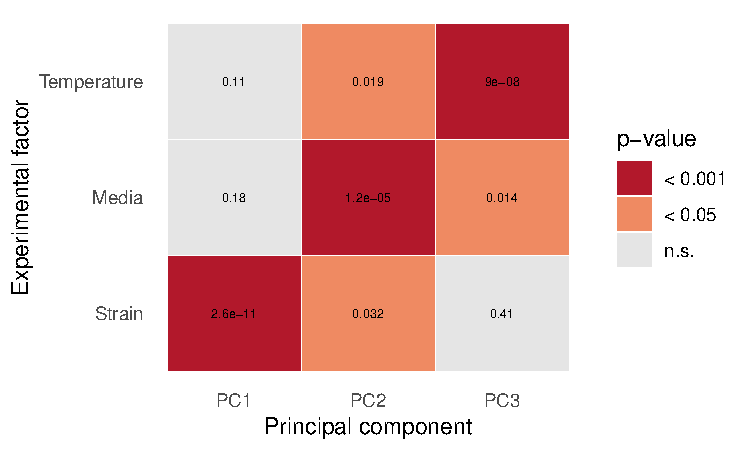
\includegraphics[keepaspectratio]{figures/anova_plot.pdf}}

}

\caption{\label{fig-anova}Heatmap of ANOVA p-values testing the
association between principal components and experimental factors.}

\end{figure}%

\begin{figure}

\centering{

\pandocbounded{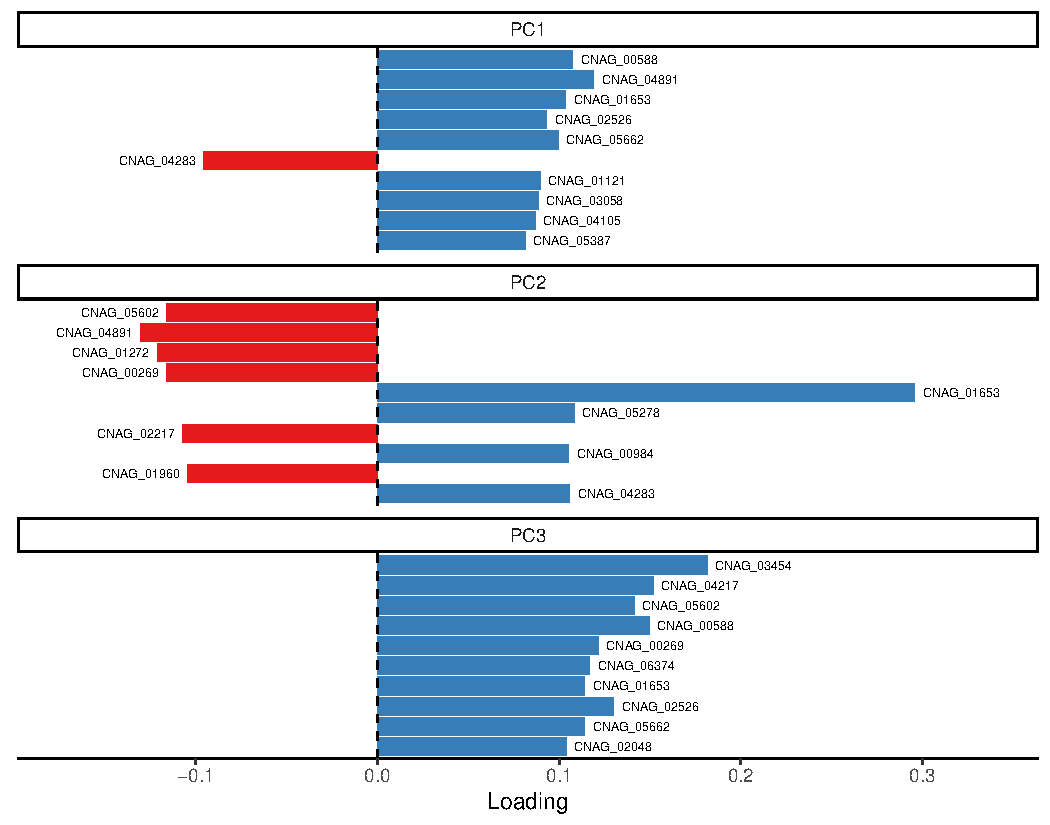
\includegraphics[keepaspectratio]{figures/pca_rlog_load_plot.pdf}}

}

\caption{\label{fig-pca-rlog-load}Barplots displaying the top 10 genes
with the highest absolute loadings for each principal component.}

\end{figure}%

The results of the pairwise ANOVA tests between the retained principal
components and experimental factors (Figure~\ref{fig-anova}) show that
PC1 primarily captures variation associated with the strain condition.
PC2 is influenced by all three experimental factors, with the strongest
association observed for the media condition. PC3 reflects separation
driven by both media and temperature, with the most significant effect
corresponding to temperature. The top 10 genes contributing most
strongly to each principal component are shown in
Figure~\ref{fig-pca-rlog-load}. Notably, CNAG\_01653 exhibits the
largest loading magnitude overall, particularly in PC2, and also shows
substantial contributions to PC1 and PC3. CNAG\_04283, which encodes the
FLC1 gene, contributes strongly to both PC1 and PC2. Another prominent
gene, CNAG\_04891, is among the top contributors to both PC1 and PC2 as
well. For PC3, CNAG\_03454 shows the highest association, followed by
CNAG\_04217 and CNAG\_00588, the latter also contributing notably to
PC1.

\section{Differential expression
analysis}\label{differential-expression-analysis}

Moving on to model fitting for DE analysis, we observed that the shrunk
dispersion estimates aligned well with the mean-dependent trend,
indicating a good overall fit (\quartosuppfigref{suppfig-dispersion}).
This pattern was more consistent in the filtered dataset, whereas in the
unfiltered dataset, the trend appeared to be overly influenced by genes
with low mean expression levels.

The contrasts used to test the significance of the model coefficients
(excluding the intercept), which correspond to the log-fold changes
(LFCs), were labelled to reflect both the main effects and interaction
terms included in the DE analysis. Main effects included ``Strain (FL)''
for the FLC1Δ strain versus WT, ``Media (YC)'', ``Media (YE)'', and
``Media (YCE)'' for the addition of CFW, EGTA, and both to YPD,
respectively, and ``Temperature (30)'' for growth at 30°C versus 37°C.
Interaction terms were labelled as ``Strain (FL) + Media (YC)'',
``Strain (FL) + Media (YE)'', and ``Strain (FL) + Media (YCE)'' to
capture the combined effect of strain and media condition, and ``Strain
(FL) + Temperature (30)'' for the interaction between strain and
temperature. As previously mentioned, our analysis focused on the
interaction terms. Unless otherwise noted, results are based on the
filtered dataset.

The (unadjusted) p-value histograms for each contrast display the
expected uniform distribution under the null hypothesis, indicating a
well-calibrated multiple testing procedure
(\quartosuppfigref{suppfig-pvalue}). Similar results were observed for
the unfiltered dataset (not shown). No outliers were detected in any
contrast. However, 129 genes (1.95\%) were automatically removed due to
low mean normalized counts during the testing of the Strain (FL) + Media
(YC) term, as part of \texttt{DESeq2}'s independent filtering procedure.
MA plots for all contrasts showed a uniform distribution of
significantly upregulated and downregulated genes across the range of
mean expression levels, suggesting that the procedure is not biased
towards highly expressed genes (\quartosuppfigref{suppfig-ma}).

\begin{table}

\caption{\label{tbl-02}Number and percentage of upregulated and
downregulated genes identified at an FDR threshold of 0.1 for each
contrast tested, along with the total number of DE genes.}

\centering{

\fontsize{7.5pt}{9.0pt}\selectfont
\begin{tabular*}{0.7\linewidth}{@{\extracolsep{\fill}}lccc}
\toprule
\textbf{Contrast} & \textbf{Upregulated} & \textbf{Downregulated} & \textbf{Total} \\ 
\midrule\addlinespace[2.5pt]
Strain (FL) + Media (YC) & 476 (37.96\%) & 778 (62.04\%) & 1254 (100\%) \\ 
Strain (FL) + Media (YCE) & 955 (42.96\%) & 1268 (57.04\%) & 2223 (100\%) \\ 
Strain (FL) + Media (YE) & 848 (48.02\%) & 918 (51.98\%) & 1766 (100\%) \\ 
Strain (FL) + Temperature (30) & 421 (36.39\%) & 736 (63.61\%) & 1157 (100\%) \\ 
\bottomrule
\end{tabular*}

}

\end{table}%

\begin{figure}

\centering{

\pandocbounded{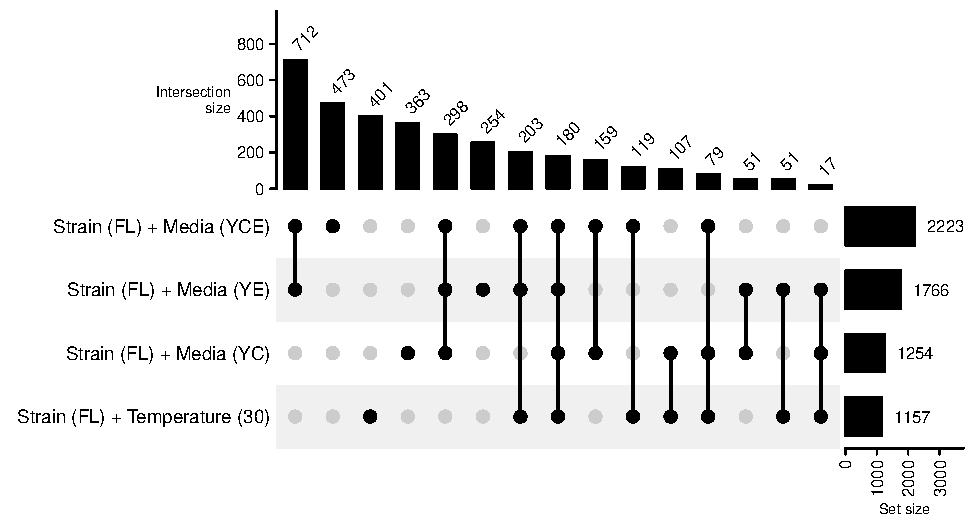
\includegraphics[keepaspectratio]{figures/upset_plot.pdf}}

}

\caption{\label{fig-upset}UpSet plot illustrating the intersections
between differentially expressed (DE) gene sets across the various
contrasts.}

\end{figure}%

The Strain (FL) + Media (YCE) contrast yielded the highest number of
differentially expressed (DE) genes (2223), while Strain (FL) +
Temperature (30) had the fewest (767) (Table~\ref{tbl-02}). All
contrasts showed more downregulated than upregulated genes. The highest
percentage of downregulated genes was observed in Strain (FL) +
Temperature (30) (63.61\%), although the contrast with the greatest
absolute number of downregulated genes was Strain (FL) + Media (YCE)
(1268). The highest proportion of upregulated genes was found in Strain
(FL) + Media (YE) (48.02\%), while the highest count of upregulated
genes overall was again seen in Strain (FL) + Media (YCE) (955)
(Table~\ref{tbl-02}). The Strain (FL) + Media (YCE) and Strain (FL) +
Media (YE) contrasts shared the highest number of differentially
expressed (DE) genes in common (712). In total, 3467 uniquely genes were
identified as differentially expressed (52.43\%), with 180 (2.72\%) of
them consistently differentially expressed across all contrasts
(Figure~\ref{fig-upset}). Strain (FL) + Media (YCE) also had the
greatest number of uniquely identified DE genes (473), i.e.~those not
shared with any other contrast. This was followed by Strain (FL) +
Temperature (30) (401), Strain (FL) + Media (YC) (363), and Strain (FL)
+ Media (YE) (254).

\begin{figure}

\centering{

\pandocbounded{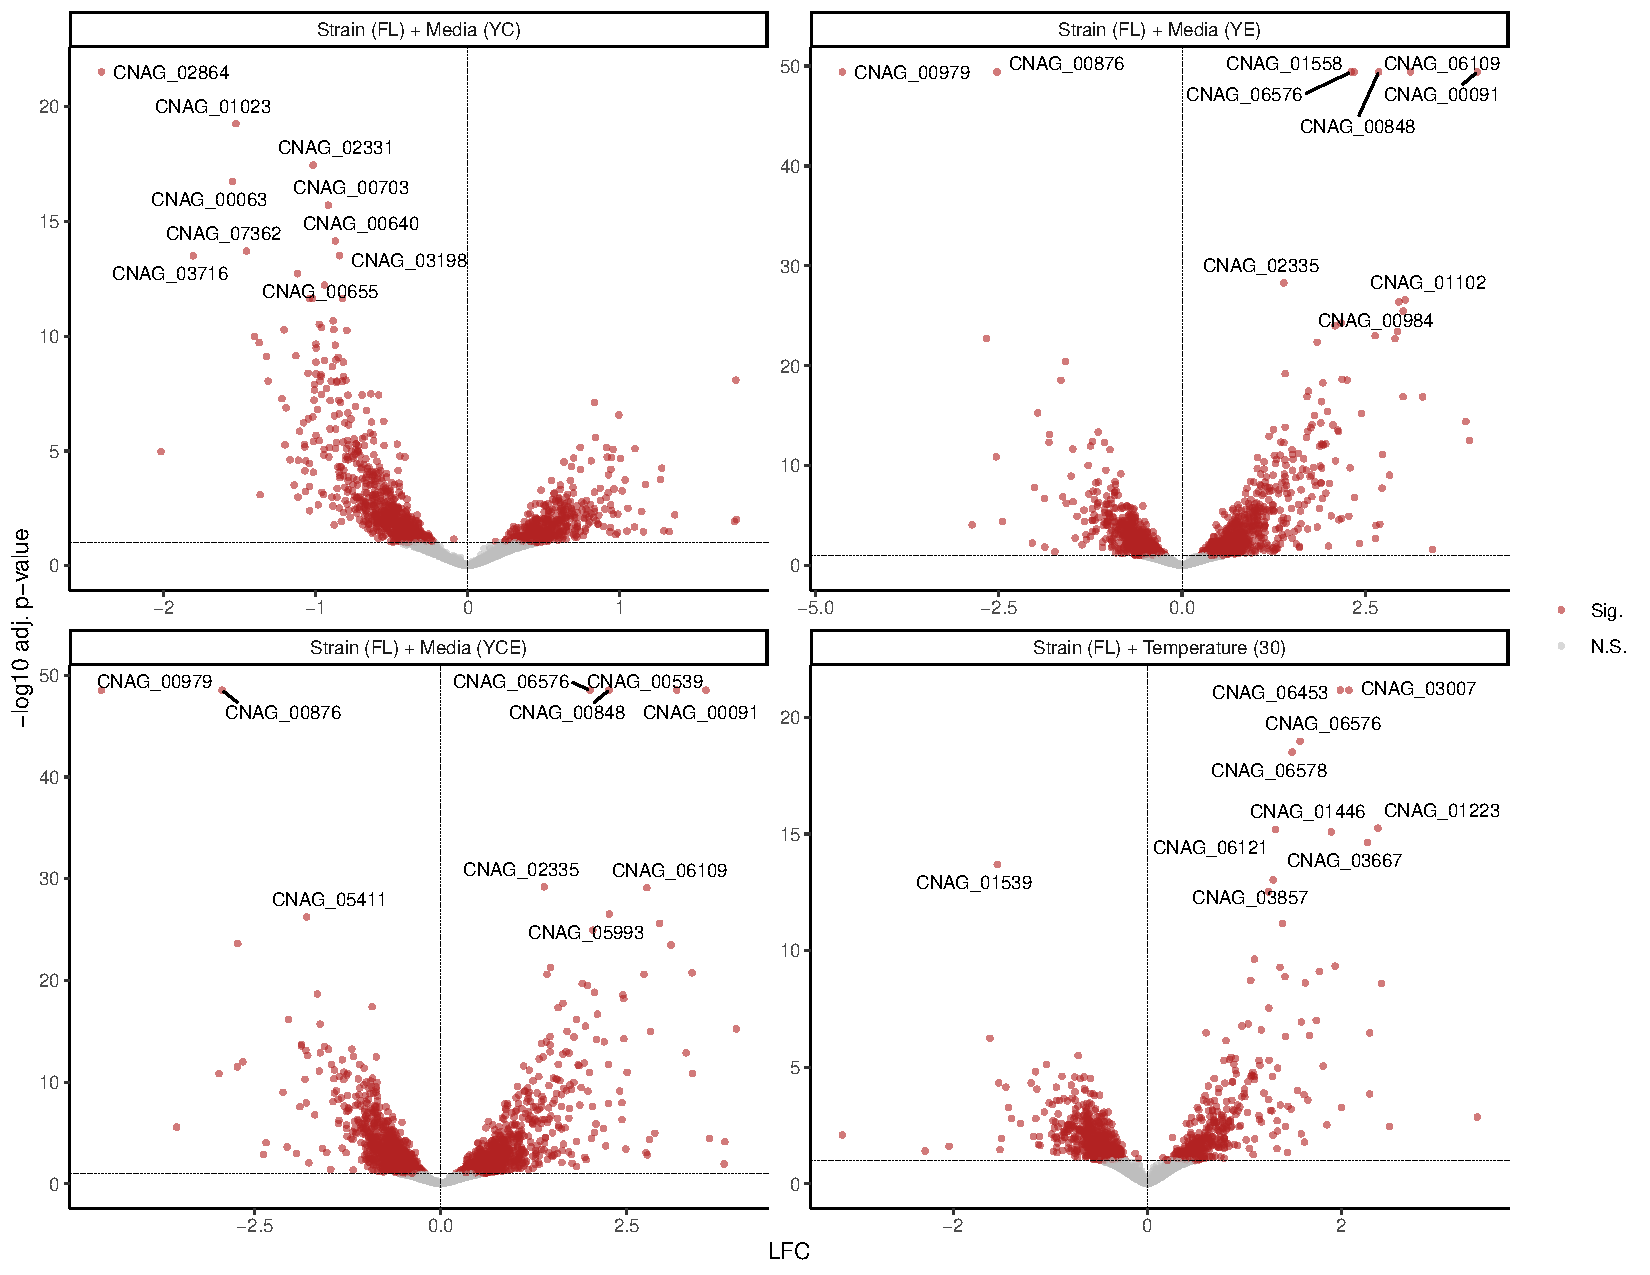
\includegraphics[keepaspectratio]{figures/volcano_plot.pdf}}

}

\caption{\label{fig-volcano}Volcano plots for each contrast highlighting
the top 10 most significant genes based on adjusted p-values and log2
fold changes.}

\end{figure}%

Figure~\ref{fig-volcano} highlights the top 10 most significant genes
for each contrast. Notably, all of the top genes for the Strain (FL) +
Media (YC) interaction were downregulated, while all but one of the top
genes for the Strain (FL) + Temperature (30) interaction were
upregulated. Gene CNAG\_06576 appeared most frequently among the top
genes, being significantly differentially expressed in all contrasts
except Strain (FL) + Media (YC). In addition, genes CNAG\_00091,
CNAG\_00848, CNAG\_00876, CNAG\_00979, and CNAG\_02335 were consistently
ranked among the top genes in both the Strain (FL) + Media (YE) and
Strain (FL) + Media (YCE) contrasts.

\section{Gene expression profiles}\label{gene-expression-profiles}

\begin{figure}

\centering{

\pandocbounded{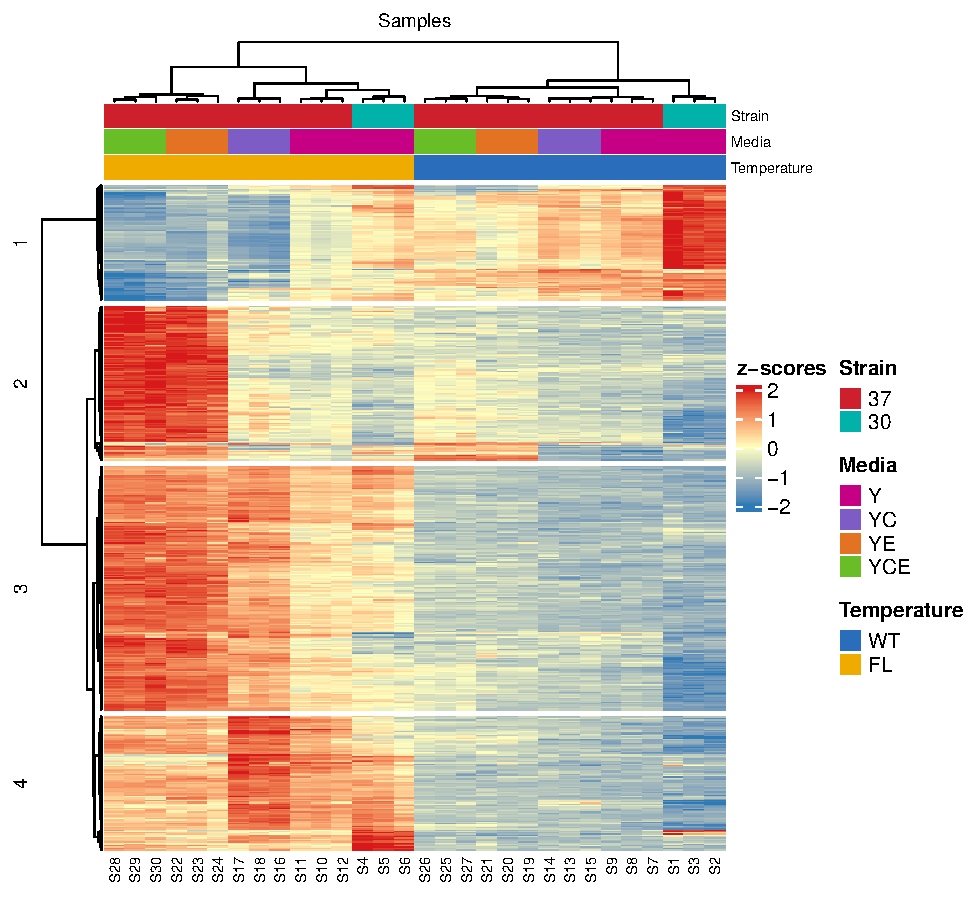
\includegraphics[keepaspectratio]{figures/heatmap_rlog.pdf}}

}

\caption{\label{fig-heatmap}Heatmap of z-scored expression levels for
the top 500 most variable genes, annotated by cluster membership and
experimental conditions.}

\end{figure}%

The optimal number of clusters for the top 500 differentially expressed
(DE) genes with the highest variance, determined by the Gap statistic,
was four when using z-scores of the rlog-transformed data
(\quartosuppfigref{suppfig-gap}). The same optimal cluster number was
obtained with VST-transformed data, whereas the \(\text{log}_2\)-CPM
transformation resulted in an uninformative single cluster, indicating
it may be less effective at capturing meaningful expression patterns in
this context.

Figure~\ref{fig-heatmap} displays a heatmap of the z-scored expression
values across the four clusters (labelled 1--4). Because the data are
z-scored, positive values indicate expression above the gene's mean
across all conditions, while negative values indicate below-average
expression. Cluster 1 is distinct, with genes showing above-average
expression in the WT strain and below-average expression in the FLC1Δ
strain, particularly under the WT-Y-30 basal condition. In contrast,
clusters 2--4 exhibit the opposite pattern, with genes generally showing
lower expression in WT and higher expression in FLC1Δ samples,
suggesting a strain-specific shift in relative expression. Within these,
cluster 2 genes tend to be upregulated in FL-YE-37 and FL-YCE-37
conditions but near or below average in other FLC1Δ combinations.
Cluster 3 follows a similar pattern but with elevated expression across
a broader range of FLC1Δ conditions. Cluster 4 displays an inverse trend
to cluster 2, with higher expression at FL-Y-30, FL-Y-37, and FL-YC-37
conditions.

\begin{figure}

\centering{

\pandocbounded{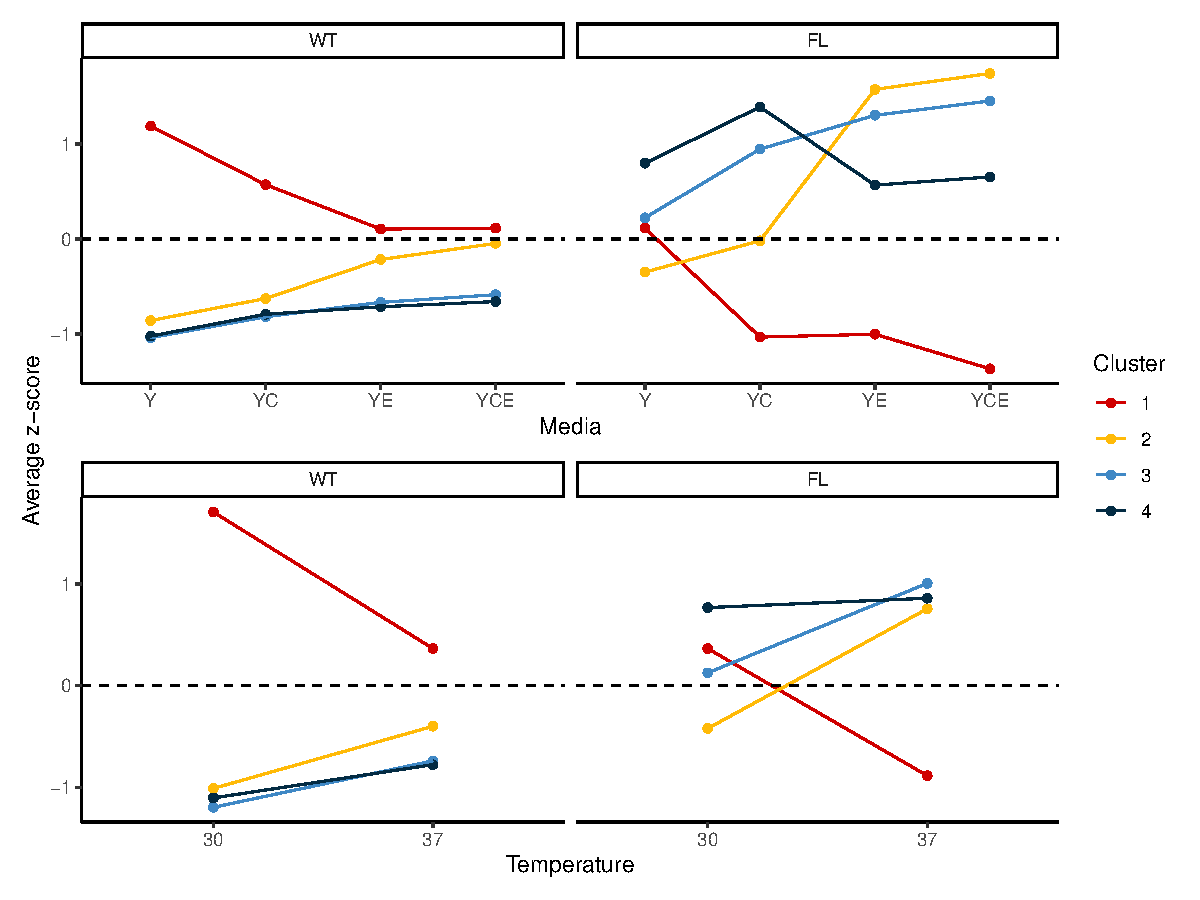
\includegraphics[keepaspectratio]{figures/cluster_profile_plot.pdf}}

}

\caption{\label{fig-profile}Line plot of average z-scored expression for
each gene cluster across growth media and temperature conditions,
faceted by strain (WT and FLC1Δ).}

\end{figure}%

Figure~\ref{fig-profile} illustrates the average z-scored expression
patterns of the four gene clusters across media and temperature
conditions, shown separately for the WT and FLC1Δ (FL) strains. In the
WT strain (top-left panel), cluster 1 genes consistently exhibit
above-average expression across all media, with the highest levels
observed in the Y media condition. Expression gradually decreases
through YC and YE to YCE, with a more pronounced drop from Y to YC than
from YE to YCE. Conversely, clusters 2, 3, and 4 show consistently
below-average expression in WT, though expression slightly increases
with the addition of CFW and EGTA.

For the FL strain (top-right panel), expression patterns invert. Cluster
1 genes are below average in all media and show a marked decrease when
CFW and EGTA are present (from Y to YC, and from YE to YCE). Clusters 2
and 3 exhibit progressively increasing expression across media,
particularly in YE and YCE. Cluster 2 displays a strong increase with
EGTA addition, whereas cluster 3 follows a similar trend but with a less
pronounced rise. Cluster 4 shows increased expression upon CFW addition
(from Y to YC and from YE to YCE), especially in the Y medium, but has
the lowest expression in EGTA-containing growth media.

Regarding temperature, in the WT strain (bottom-left panel), cluster 1
genes remain above average at both 30°C and 37°C, but with reduced
expression at 37°C. Clusters 2--4 remain below average, though
expression levels increase with temperature. In the FL strain
(bottom-right panel), the patterns again invert: cluster 1 genes show
near or below-average expression, decreasing further at 37°C. Clusters 2
and 3 show near or above-average expression that increases with
temperature, while cluster 4 maintains above-average expression with
little change across temperatures.

\begin{figure}

\centering{

\pandocbounded{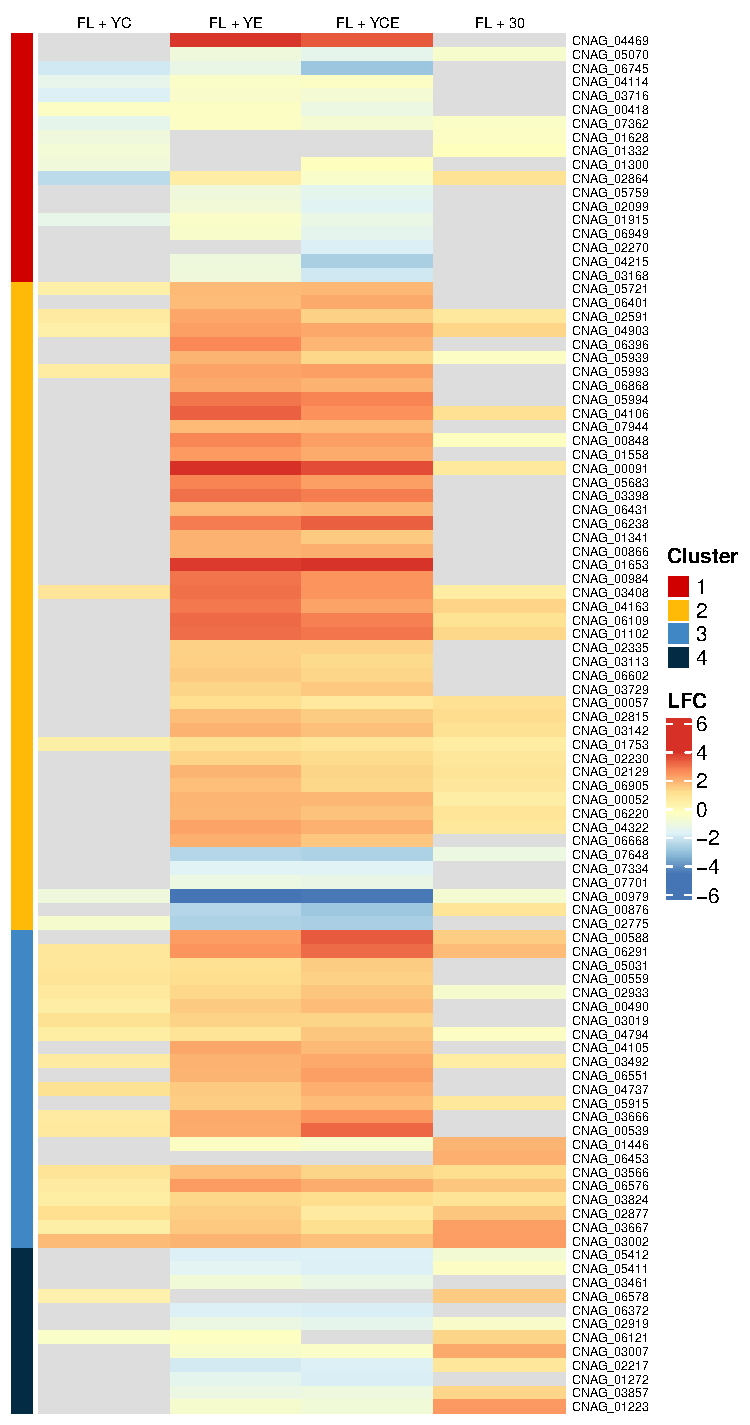
\includegraphics[keepaspectratio]{figures/heatmap_lfc.pdf}}

}

\caption{\label{fig-heatmap-lfc}Heatmap of log2 fold changes for the top
100 ranked genes across all contrasts, with cluster membership
indicated.}

\end{figure}%

\section{Gene prioritization}\label{gene-prioritization}

To prioritise the most informative genes, we ranked the 500 genes used
for clustering based on two criteria: smallest adjusted p-value and
largest absolute log2 fold change (LFC), then computed an average rank
across both metrics. The top 100 genes according to this combined
ranking are shown in Figure~\ref{fig-heatmap-lfc}, which presents a
heatmap of their LFCs across all contrasts alongside their cluster
membership. This plot provides a comprehensive summary, integrating
statistical significance, expression changes, and clustering results to
identify candidate genes of interest. For example, CNAG\_04469, which
appears near the top of the heatmap, is significantly differentially
expressed in the interaction between strain and media at the YE and YCE
levels, but not at other contrasts. In both cases, this gene is
upregulated in the FL strain relative to the WT-Y-37 reference. As a
member of cluster 2, its expression profile aligns with that described
for cluster 2 genes in Figure~\ref{fig-profile}. Additionally, many of
the top-ranked genes exhibit significant LFCs specifically in the YE and
YCE conditions, with significance in one condition often accompanied by
significance in the other.

\bookmarksetup{startatroot}

\chapter{Conclusions}\label{sec-conclusions}

This report presents the analysis of RNA-Seq data from an experiment
investigating the response of \emph{Cryptococcus neoformans} to cell
wall stress across various environmental and genetic conditions,
focusing on the FLC1 gene, a promising antifungal drug target. The study
aimed to provide statistically robust insights into transcriptomic
responses to combinations of growth media (CFW, EGTA, or both),
temperature (30°C and 37°C), and the presence or absence of FLC1. The
objectives were to assess replicate consistency, explore broad
expression patterns among samples, identify differentially expressed
genes across conditions, and reveal structured expression profiles
within those genes.

Replicates clustered closely in PCA, indicating good biological
consistency. Samples grown in YPD and YPD + CFW, as well as YPD + EGTA
and YPD + CFW + EGTA, clustered together, but similarity varied by
strain. In the FLC1Δ strain, adding CFW caused greater expression
changes than in WT, with distinct profiles especially in YPD + CFW.
Genes driving these patterns included CNAG\_04283 (FLC1), CNAG\_01653,
CNAG\_04891, and CNAG\_00588. At 37°C, the FLC1Δ strain showed more
expression variation across media, while at 30°C, greater overall
divergence was observed. However, PCA loadings alone do not confirm
differential expression for individual genes.

About 52.4\% of genes (3,467) were differentially expressed in
strain-media and strain-temperature contrasts relative to WT at 37°C in
YPD. The greatest number of DE genes occurred in the FLC1Δ strain at
37°C with YPD + CFW + EGTA, mostly downregulated, with the highest
downregulation (62\%) seen in FLC1Δ at 37°C in YPD + CFW. Gene
CNAG\_06576 was consistently significant, generally upregulated except
for downregulation in that latter condition. Clustering the top 500 most
variable DE genes identified four groups: cluster 1 genes were expressed
above average in WT and below average in FLC1Δ, while clusters 2--4
showed the opposite pattern, indicating a strain-specific expression
shift. Cluster 1 genes had higher expression under basal conditions
(YPD, 30°C) and lower under stress (CFW, EGTA, 37°C), with clusters 2--4
displaying inverse trends more marked in FLC1Δ. Notably, cluster 4 genes
decreased expression with EGTA and were largely unaffected by
temperature. In addition, a ranked list of the top 100 DE genes with
cluster annotations is provided for future study.

One limitation of this analysis is the reliance on a single algorithm
for detecting differentially expressed genes, specifically the method
implemented in the \texttt{DESeq2} package. The robustness of the
findings presented in this report could be further evaluated by applying
alternative differential expression analysis methods.

\bookmarksetup{startatroot}

\chapter*{References}\label{references}
\addcontentsline{toc}{chapter}{References}

\markboth{References}{References}

\phantomsection\label{refs}
\begin{CSLReferences}{0}{1}
\bibitem[\citeproctext]{ref-may2016cryptococcus}
\CSLLeftMargin{1. }%
\CSLRightInline{May RC, Stone NR, Wiesner DL, Bicanic T, Nielsen K.
Cryptococcus: From environmental saprophyte to global pathogen. Nature
Reviews Microbiology. 2016;14(2):106--17. }

\bibitem[\citeproctext]{ref-stempinski2022cryptococcus}
\CSLLeftMargin{2. }%
\CSLRightInline{Stempinski PR, Goughenour KD, Plooy LM du, Alspaugh JA,
Olszewski MA, Kozubowski L. The cryptococcus neoformans Flc1 homologue
controls calcium homeostasis and confers fungal pathogenicity in the
infected hosts. Mbio. 2022;13(5):e02253--22. }

\bibitem[\citeproctext]{ref-wang2009rna}
\CSLLeftMargin{3. }%
\CSLRightInline{Wang Z, Gerstein M, Snyder M. RNA-seq: A revolutionary
tool for transcriptomics. Nature reviews genetics. 2009;10(1):57--63. }

\bibitem[\citeproctext]{ref-chen2016from}
\CSLLeftMargin{4. }%
\CSLRightInline{Chen Y, Lun TLL, Smyth GK.
\href{https://doi.org/10.12688/f1000research.8987.2}{From reads to genes
to pathways: Differential expression analysis of RNA-seq experiments
using rsubread and the edgeR quasi-likelihood pipeline}. F1000Research.
2016;5(1438). }

\bibitem[\citeproctext]{ref-sha2015effect}
\CSLLeftMargin{5. }%
\CSLRightInline{Sha Y, Phan JH, Wang MD. Effect of low-expression gene
filtering on detection of differentially expressed genes in RNA-seq
data. In: 2015 37th annual international conference of the IEEE
engineering in medicine and biology society (EMBC). IEEE; 2015. p.
6461--4. }

\bibitem[\citeproctext]{ref-bourgon2010independent}
\CSLLeftMargin{6. }%
\CSLRightInline{Bourgon R, Gentleman R, Huber W. Independent filtering
increases detection power for high-throughput experiments. Proceedings
of the National Academy of Sciences. 2010;107(21):9546--51. }

\bibitem[\citeproctext]{ref-chen2025edgeR}
\CSLLeftMargin{7. }%
\CSLRightInline{Chen Y, Chen L, Lun ATL, Baldoni P, Smyth GK.
\href{https://doi.org/10.1093/nar/gkaf018}{{edgeR} v4: Powerful
differential analysis of sequencing data with expanded functionality and
improved support for small counts and larger datasets}. Nucleic Acids
Research. 2025;53(2):gkaf018. }

\bibitem[\citeproctext]{ref-gierlinski2015statistical}
\CSLLeftMargin{8. }%
\CSLRightInline{Gierliński M, Cole C, Schofield P, Schurch NJ, Sherstnev
A, Singh V, et al. Statistical models for RNA-seq data derived from a
two-condition 48-replicate experiment. Bioinformatics.
2015;31(22):3625--30. }

\bibitem[\citeproctext]{ref-dillies2012a}
\CSLLeftMargin{9. }%
\CSLRightInline{Dillies MA, Rau A, Aubert J, Hennequet-Antier C,
Jeanmougin M, Servant N, et al. A comprehensive evaluation of
normalization methods for illumina high-throughput RNA sequencing data
analysis. Briefings in Bioinformatics {[}Internet{]}. 2012
Sep;14(6):671--83. Available from:
\url{https://doi.org/10.1093/bib/bbs046}}

\bibitem[\citeproctext]{ref-robinson2010scaling}
\CSLLeftMargin{10. }%
\CSLRightInline{Robinson MD, Oshlack A. A scaling normalization method
for differential expression analysis of RNA-seq data. Genome biology.
2010;11:1--9. }

\bibitem[\citeproctext]{ref-anders2010differential}
\CSLLeftMargin{11. }%
\CSLRightInline{Anders S, Huber W. Differential expression analysis for
sequence count data. Nature Precedings. 2010;1--1. }

\bibitem[\citeproctext]{ref-love2014moderated}
\CSLLeftMargin{12. }%
\CSLRightInline{Love MI, Huber W, Anders S. Moderated estimation of fold
change and dispersion for RNA-seq data with DESeq2. Genome biology.
2014;15:1--21. }

\bibitem[\citeproctext]{ref-hafemeister2019normalization}
\CSLLeftMargin{13. }%
\CSLRightInline{Hafemeister C, Satija R. Normalization and variance
stabilization of single-cell RNA-seq data using regularized negative
binomial regression. Genome biology. 2019;20(1):296. }

\bibitem[\citeproctext]{ref-dinno2009exploring}
\CSLLeftMargin{14. }%
\CSLRightInline{Dinno A. Exploring the sensitivity of horn's parallel
analysis to the distributional form of random data. Multivariate
behavioral research. 2009;44(3):362--88. }

\bibitem[\citeproctext]{ref-zhu2019heavy}
\CSLLeftMargin{15. }%
\CSLRightInline{Zhu A, Ibrahim JG, Love MI. Heavy-tailed prior
distributions for sequence count data: Removing the noise and preserving
large differences. Bioinformatics. 2019;35(12):2084--92. }

\bibitem[\citeproctext]{ref-meeta2021hbctraining}
\CSLLeftMargin{16. }%
\CSLRightInline{Mistry M, Piper M, Liu J, Khetani R.
Hbctraining/DGE\_workshop\_salmon\_online: Differential gene expression
workshop lessons from HCBC (first release) {[}Internet{]}. Zenodo; 2021.
Available from: \url{https://doi.org/10.5281/zenodo.4783481}}

\bibitem[\citeproctext]{ref-benjamini1995controlling}
\CSLLeftMargin{17. }%
\CSLRightInline{Benjamini Y, Hochberg Y. Controlling the false discovery
rate: A practical and powerful approach to multiple testing. Journal of
the Royal statistical society: series B (Methodological).
1995;57(1):289--300. }

\bibitem[\citeproctext]{ref-psu2025stat}
\CSLLeftMargin{18. }%
\CSLRightInline{The Pennsylvania State University. STAT 555: Statistical
analysis of genomics data.
\url{https://online.stat.psu.edu/statprogram/stat555}; 2025. }

\bibitem[\citeproctext]{ref-tibshirani2001estimating}
\CSLLeftMargin{19. }%
\CSLRightInline{Tibshirani R, Walther G, Hastie T. Estimating the number
of clusters in a data set via the gap statistic. Journal of the royal
statistical society: series b (statistical methodology).
2001;63(2):411--23. }

\end{CSLReferences}

\bookmarksetup{startatroot}

\chapter*{Appendix}\label{appendix}
\addcontentsline{toc}{chapter}{Appendix}

\markboth{Appendix}{Appendix}

\section*{Word count}\label{word-count}
\addcontentsline{toc}{section}{Word count}

\markright{Word count}

The total word count on the main text is 4998:


\includegraphics[width=0.4\linewidth,height=\textheight,keepaspectratio]{figures/wordcount.png}

\section*{Suplementary figures}\label{suplementary-figures}
\addcontentsline{toc}{section}{Suplementary figures}

\markright{Suplementary figures}

\begin{suppfig}

\centering{

\pandocbounded{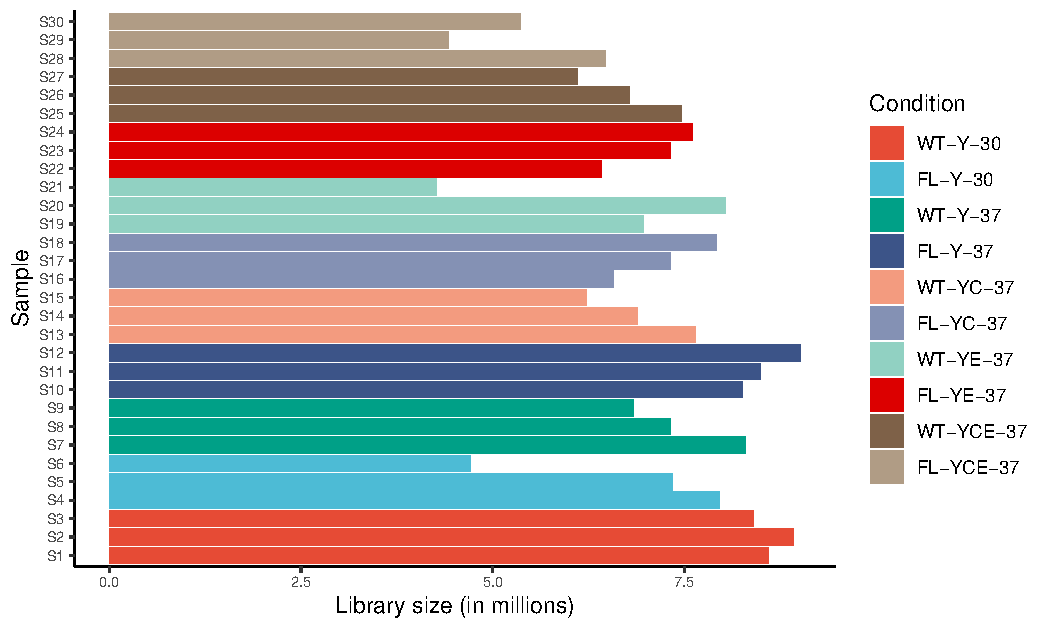
\includegraphics[keepaspectratio]{figures/lib_sizes.pdf}}

}

\caption{\label{suppfig-libsize}Barplot showing the total number of
sequenced reads (in millions) per sample, with bars coloured by
experimental condition.}

\end{suppfig}%

\begin{suppfig}

\centering{

\pandocbounded{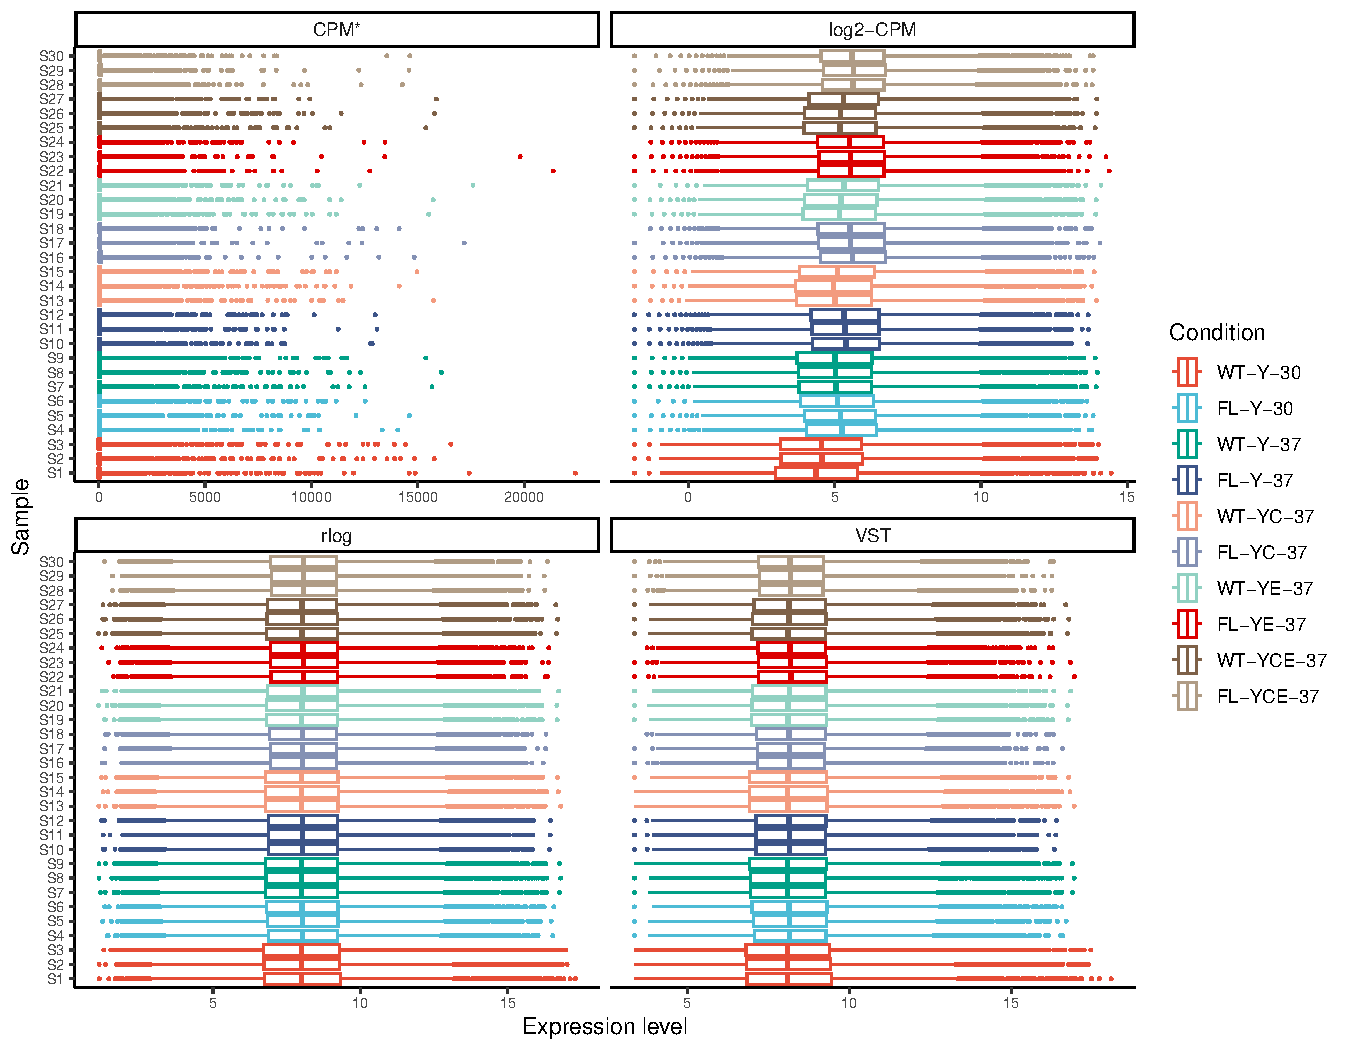
\includegraphics[keepaspectratio]{figures/transformed_filter_boxplot.pdf}}

}

\caption{\label{suppfig-boxplots}Boxplots of gene expression values by
sample, coloured by experimental condition and faceted by transformation
method. Note that CPM* denotes normalisation only, without variance
stabilisation.}

\end{suppfig}%

\begin{suppfig}

\centering{

\pandocbounded{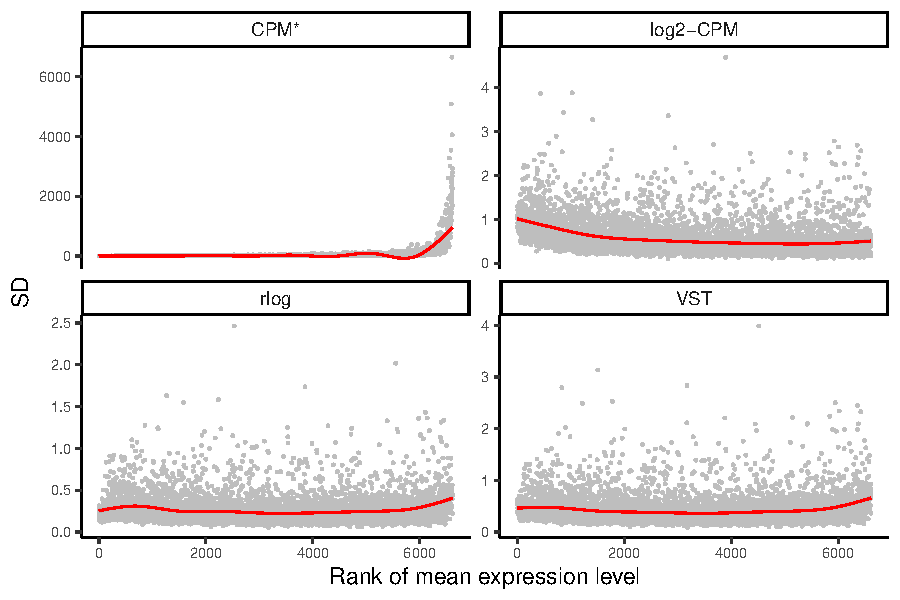
\includegraphics[keepaspectratio]{figures/meansd_plot.pdf}}

}

\caption{\label{suppfig-meansd}Mean versus standard deviation plot of
gene expression values, faceted by transformation method. The red line
indicates the mean-dependent trend in standard deviation. CPM* lacks
variance stabilisation, as reflected in its stronger mean--SD
dependence.}

\end{suppfig}%

\begin{suppfig}

\centering{

\pandocbounded{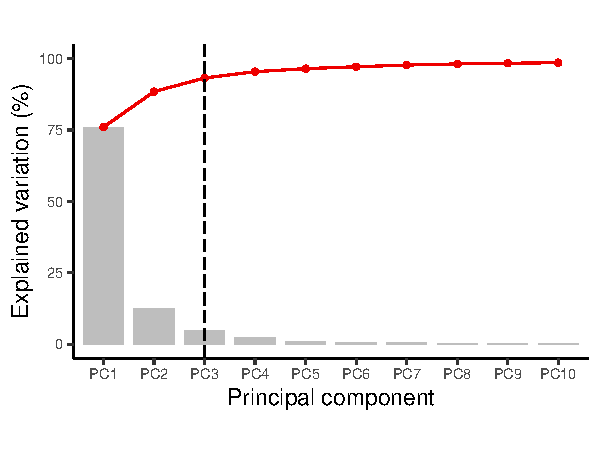
\includegraphics[keepaspectratio]{figures/screeplot_rlog.pdf}}

}

\caption{\label{suppfig-scree}Scree plot of the rlog-transformed data
showing the number of retained principal components based on parallel
analysis.}

\end{suppfig}%

\begin{suppfig}

\centering{

\pandocbounded{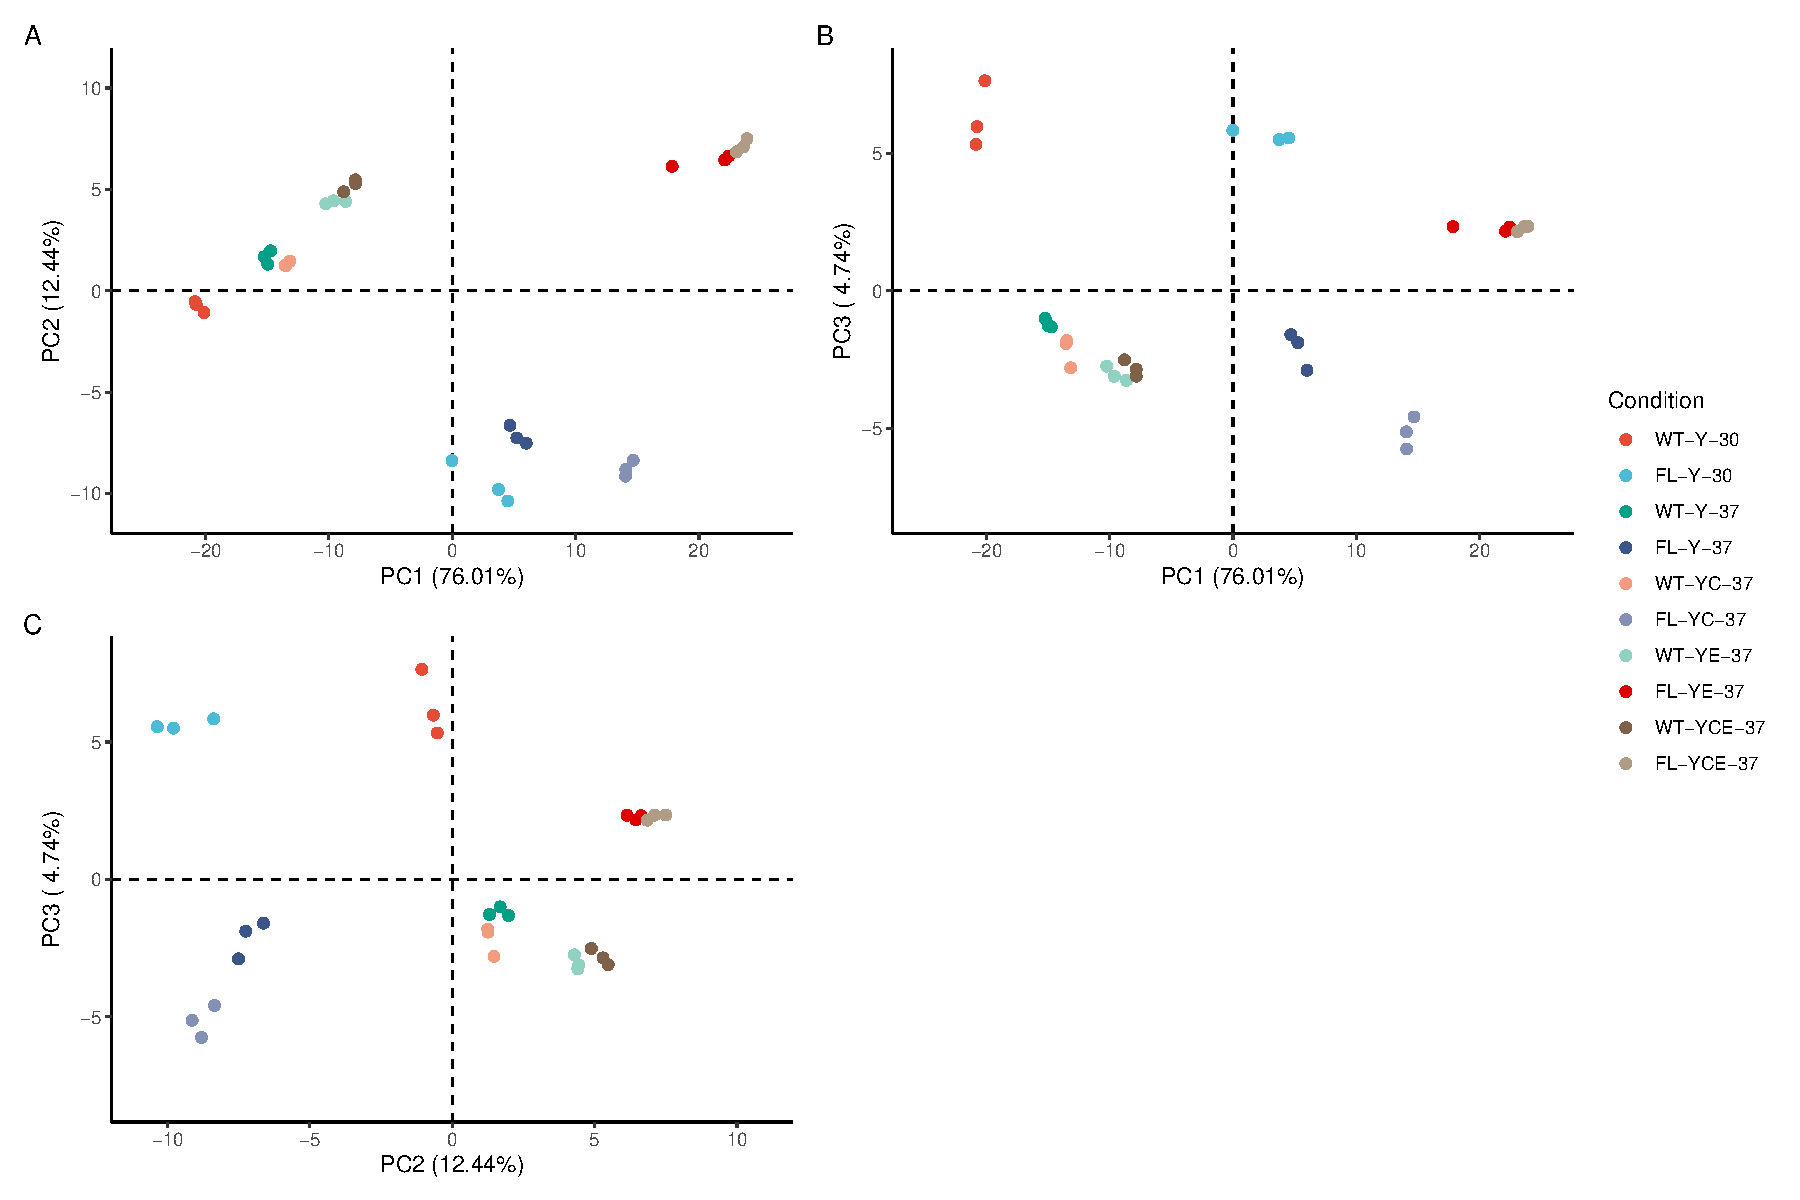
\includegraphics[keepaspectratio]{figures/pca_rlog_plot.pdf}}

}

\caption{\label{suppfig-pca-rlog}Samples projected onto pairwise
combinations of retained principal components from the rlog-transformed
data, coloured by experimental condition.}

\end{suppfig}%

\begin{suppfig}

\centering{

\pandocbounded{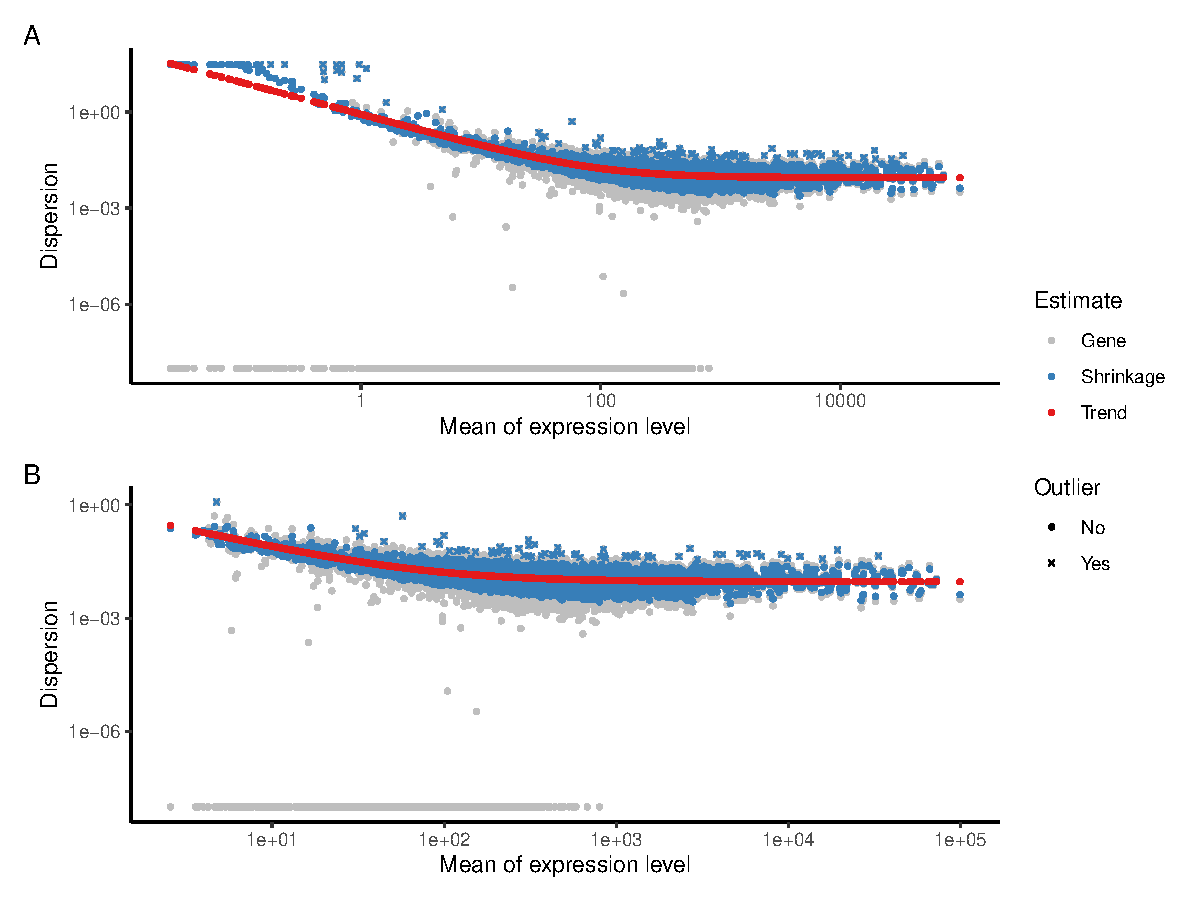
\includegraphics[keepaspectratio]{figures/dispersion_plot.pdf}}

}

\caption{\label{suppfig-dispersion}Dispersion estimates plotted against
mean expression levels. Gray points represent gene-wise dispersion
estimates, blue points show shrinkage-based estimates, and the red line
indicates the mean-dependent trend. Panel (A) corresponds to unfiltered
data, while panel (B) shows filtered data.}

\end{suppfig}%

\begin{suppfig}

\centering{

\pandocbounded{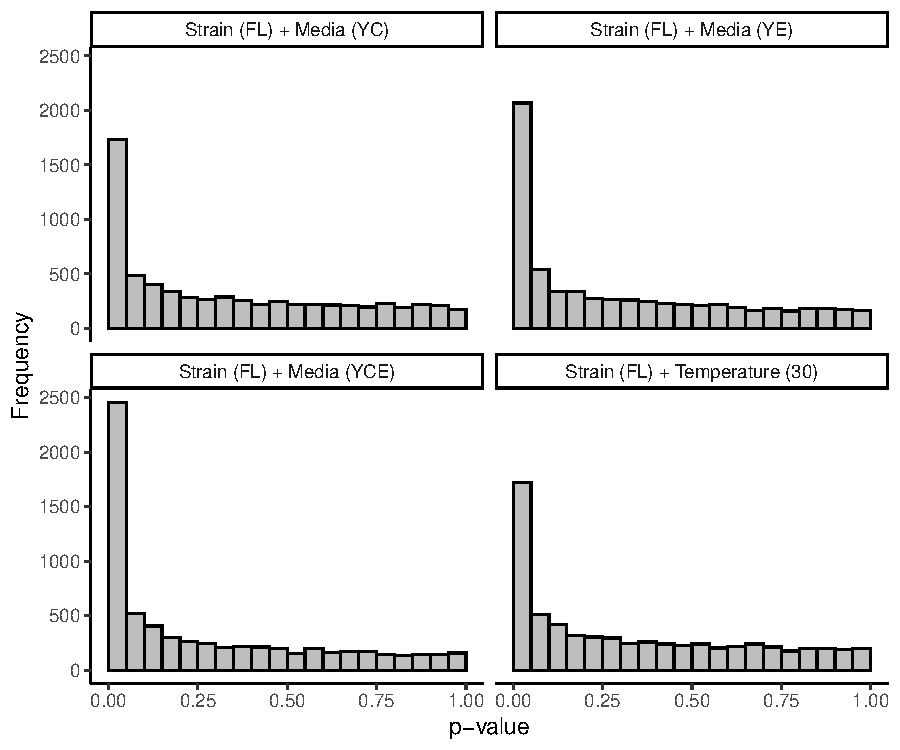
\includegraphics[keepaspectratio]{figures/pvalue_hist.pdf}}

}

\caption{\label{suppfig-pvalue}Histograms of unadjusted p-values for
each contrast.}

\end{suppfig}%

\begin{suppfig}

\centering{

\pandocbounded{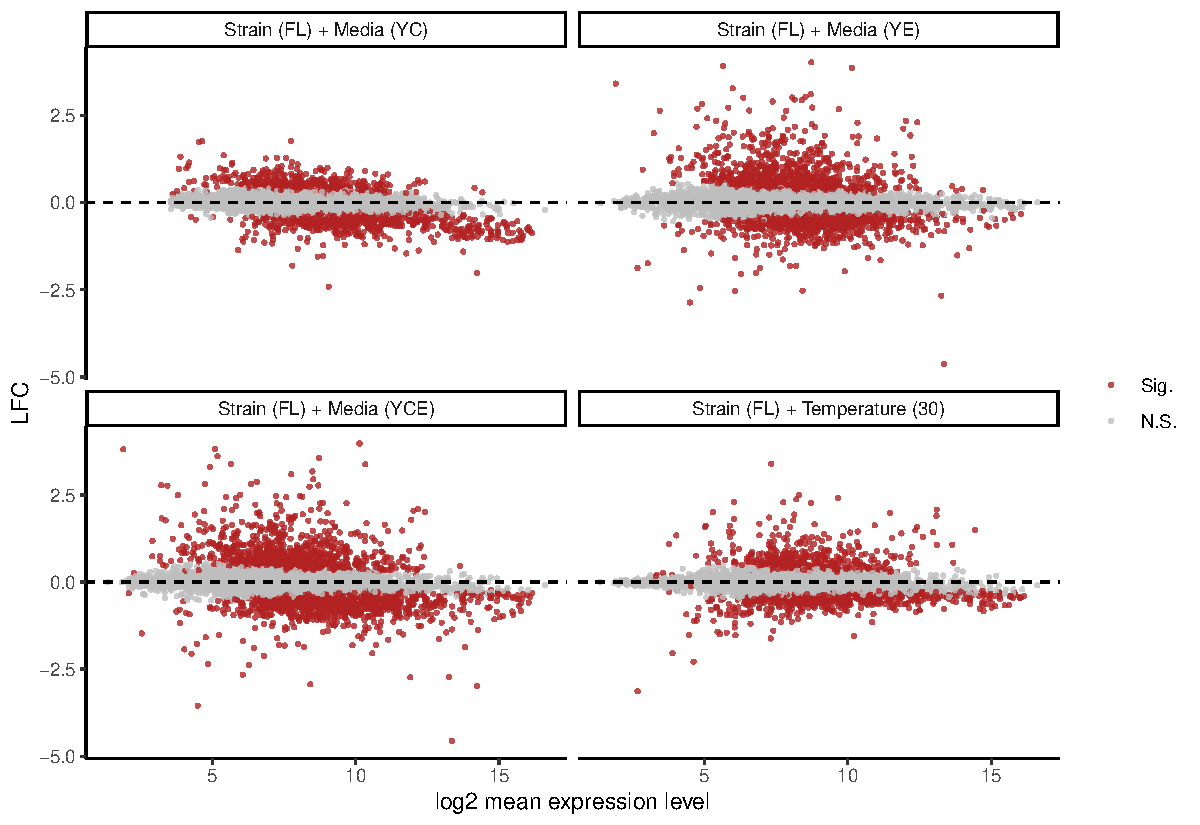
\includegraphics[keepaspectratio]{figures/ma_plot.pdf}}

}

\caption{\label{suppfig-ma}MA plots displaying log2 fold change (LFC)
estimates with shrinkage across mean expression levels for each
contrast. Red points indicate significantly differentially expressed
genes, while gray points represent non-significant genes.}

\end{suppfig}%

\begin{suppfig}

\centering{

\pandocbounded{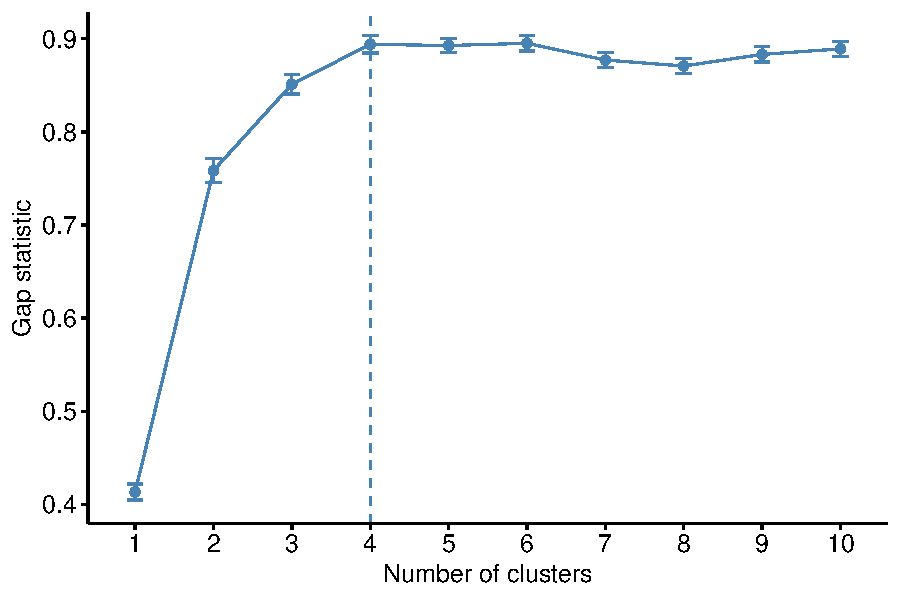
\includegraphics[keepaspectratio]{figures/gap_plot.pdf}}

}

\caption{\label{suppfig-gap}Gap statistic plot showing the optimal
number of clusters for the top 500 most variable genes based on
rlog-transformed data. The optimal cluster number is indicated by the
vertical dashed line.}

\end{suppfig}%




\end{document}
